\documentclass{mrl}

\title{Оценка безопасности криптовалюты и её анонимности в постквантовом мире}
\authors{Адам Корбо (Adam Corbo)\footnote{\texttt{adamryancorbo@gmail.com}}, Митчел ``Isthmus'' Кравиц-Тайер (Mitchell Krawiec-Thayer)\footnote{\texttt{Isthmus@getmonero.org} или \texttt{IsthmusCrypto@protonmail.com}}, \\ Брэндон Дж. Гуделл (Brandon G Goodell)\footnote{\texttt{surae@getmonero.org}}}
\affiliations{Insight и Исследовательская лаборатория Monero (Monero Research Lab)}
\date{Сентябрь 2020}

% font stuff
\usepackage[official]{eurosym}
\usepackage{amssymb}
\usepackage{braket}
\usepackage{comment}
\usepackage[T1]{fontenc} % Allows direct pipes
\usepackage[titletoc]{appendix}
\DeclareSymbolFont{bbold}{U}{bbold}{m}{n}
\DeclareSymbolFontAlphabet{\mathbbold}{bbold}
\usepackage[utf8]{inputenc}
\usepackage[T2A]{fontenc}
\usepackage[english,russian]{babel}

% math stuff
\newtheorem{thm}{Theorem}[section]
\newtheorem{lem}[thm]{Lemma}
\newtheorem{cor}[thm]{Corollary}
\newtheorem{ex}[thm]{Example}
\newtheorem{ass}[thm]{Assumption}

% Increase margin size and in-margin todo-notes. Comment this line 15-19 out before pub
\usepackage{todonotes}
% If margin notes are too cramped use the following or something like it (or just read the source)
%\paperwidth=\dimexpr \paperwidth + 6cm\relax
%\oddsidemargin=\dimexpr\oddsidemargin + 3cm\relax
%\evensidemargin=\dimexpr\evensidemargin + 3cm\relax
%\marginparwidth=\dimexpr \marginparwidth + 3cm\relax
% Line numbers. Comment these out before pub
\usepackage{lineno}
% \linenumbers
\usepackage{enumerate}

% Watermark stuff
%\usepackage{draftwatermark}
%\SetWatermarkScale{4}
%\SetWatermarkLightness{0.95}

% Rotations?
\usepackage{graphicx}
\usepackage{bm}
\newcommand{\flipleadsto}{\mathbin{\rotatebox[origin=c]{180}{$\leadsto$}}}
\newcommand{\mnote}[1]{\todo[color=blue!20, inline, size=\small]{M notes: #1}}
\newcommand{\bnote}[1]{\todo[color=green!20, inline, size=\small]{B notes: #1}}
\newcommand{\anote}[1]{\todo[color=yellow!20, inline, size=\small]{A notes: #1}}

\type{ТЕХНИЧЕСКАЯ ЗАПИСКА}
\ident{MRL-00XX.0}

\begin{document}
\vspace{-0.25cm}
\begin{abstract}

Мы анализируем некоторые свойства безопасности протокола Monero в контексте возможностей квантовых компьютеров и используемых ими алгоритмов, включая алгоритм Шнорра, алгоритм Гровера, алгоритм Саймона, квантовый дифференциальный криптоанализ и квантовый доступ к случайным оракулам. Нами подробно описаны несколько теоретических уязвимостей: возможность выведения приватных ключей на основе публичных ключей, возможность выведения ключей на основе одноразовых адресов, возможность выявления действительного входа в кольцевых подписях, нарушение сбалансированности транзакций, раскрытие сумм транзакций, связывание множества транзакций с одним и тем же адресом, расшифровка идентификаторов платежей, а также конфликты хешей. Нами также рассматриваются несколько возможных постквантовых настроек: использование криптографии на основе решёток, многовариантной криптографии, криптографии на основе хеширования, а также криптографии на эллиптических кривых с суперсингулярной изогенией. Среди альтернативных протоколов рассматриваются ZK-STARKs, MatRiCT, Raptor-512 и RingRainbow. На основе размера подписи/доказательства, размера публичных ключей, времени генерирования и верификации нами исследуются общие компромиссы и сравниваются возможные протоколы. Для заинтересованного читателя нами предлагается простой вариант реализации алгоритмов Шнорра, Гровера и Саймона на языке Python, а также результаты, полученные нами для коммерческого квантового аппаратного обеспечения.\\ \url{https://github.com/insight-decentralized-consensus-lab/post-quantum-monero}
 
\end{abstract}

%\tableofcontents
%\thispagestyle{empty}
%\cleardoublepage

\section{Вступление}

В основе безопасности существующих на сегодняшний день криптовалют, таких как Bitcoin, Ethereum, Monero и Zcash, лежит решение вычислительно сложных задач. К таким способам защиты принадлежит, как кажется, повсеместно используемый метод, основанный на сложности решения задачи дискретного логарифмирования, который применяется по крайней мере со времени публикации работы \cite{diffie1976new}. Все перечисленные криптовалютные протоколы как минимум частично опираются на сложность решения задачи дискретного логарифмирования, которая является базисом, обеспечивающим защиту на уровне классических компьютеров (см. работы \cite{masteringbitcoin}, \cite{masteringethereum}, \cite{masteringmonero} и \cite{zcashprotocol}). Но существуют квантовые алгоритмы, позволяющие решить эту задачу за полиномиальное время при наличии достаточно производительного квантового аппаратного обеспечения. Технически эти алгоритмы можно использовать и с классическим компьютером, но это будет неэффективно при отсутствии доступа к такому аппаратному обеспечению.

Мы анализируем безопасность протоколов блокчейна в контексте нескольких квантовых алгоритмов, используя Monero в качестве практического примера. Отмеченные уязвимости, такие как возможность генерирования ключей, характерны для многих монет, в основе которых лежит криптография на эллиптических кривых, и было бы ошибочно считать их присущими исключительно Monero с точки зрения полученных результатов.

В течение нескольких последних десятилетий теория квантовых алгоритмов и методов стремительно развивалась. Мы считаем, что формальный анализ влияния на безопасность существующих протоколов, а также обсуждение долгосрочного ухода от использования протоколов, не защищённых от атак обладающего квантовыми мощностями злоумышленника, уже представляются запоздалыми. Настоящая техническая записка не может считаться исчерпывающей. Появляется всё больше квантовых алгоритмов и соответствующих возможностей. Кроме того, уже могут существовать методы, пока не известные широкой публике.

Криптографами были разработаны протоколы для использования с классическими компьютерами, которые в равной степени устойчивы к злонамеренному применению квантовых методов, и эти протоколы могут быть адаптированы для Monero. У каждого подхода есть свои преимущества, недостатки, и для каждого из них характерны сложности, связанные с требуемым пространством/временем. Некоторые из них описываются нами в Разделе \ref{sec:altprot}. 

Рассуждения на тему, появятся ли когда-нибудь квантовые компьютеры в реальности, и если да, то когда это произойдёт, не являются темой этой технической записки. Насколько нам известно, в настоящее время не существует приемлемых постквантовых анонимных криптовалют, а это значит, что на уровне сегодняшней технологии можно говорить лишь о краткосрочной или среднесрочной финансовой анонимности. Первый протокол, который обеспечит анонимность при условии применения злоумышленником квантовых методов, займёт сильные позиции даже в предквантовом мире.

\subsection{Предварительные условия, информация и терминология}

Мы обозначаем сцепление строк как $\mid \mid$. В случае с конечным неупорядоченным множеством $X$, где $\left|X\right| = n$, следует отметить, что мы можем произвольно определять элементы $X$ и допускать, что $X = \left[n\right] = \left\{1, 2, \ldots, n\right\}$, без какого-либо ущерба для общности. Мы обозначаем криптографические хеш-функции, используя $\mathcal{H}$.

Мы говорим, что две транзакции являются \textit{несвязываемыми}, если стороне, не являющейся получающей стороной, трудно определить, имеют ли две транзакции одно и того же получателя или нет. Мы говорим, что подписанта транзакции \textit{определить нельзя}, если стороне, не являющейся отправляющей стороной, трудно определить отправителя транзакции. Мы называем транзакции \textit{конфиденциальными}, если стороне, не являющейся получающей и не являющейся отправляющей стороной, трудно определить сумму транзакции.

Если мы говорим о \textit{классическом злоумышленнике}, которого сокращённо обозначаем CA, то мы имеем в виду, что у такого злоумышленника есть доступ только к вероятностной машине Тьюринга. Если мы говорим о \textit{квантовом злоумышленнике}, которого сокращёно обозначаем QA, мы имеем в виду, что такой злоумышленник имеет доступ к любому устройству (устройствам), способному эффективно выполнять квантовые алгоритмы и обладающему достаточной степенью масштабируемости, чтобы конкретно угрожать безопасности криптографических примитивов, лежащих в основе протокола Monero. Это не определяется каким-то волшебным количеством кубитов или какой-либо определённой конфигурацией; скорее, это касается способности выгодно использовать такие методы, как алгоритм Шнорра (см. работу \cite{Shor1994algorithms}), алгоритм Гровера (см. работу \cite{grover1996fast}) и алгоритм Саймона (см. работу \cite{simon1997power}), и делать это достаточно эффективно, чтобы обойти протокол Monero.

Во всех случаях мы предполагаем, что QA и CA имеют доступ к публичным данным блокчейна. В некоторых разделах мы отмечаем, что проведение атаки требует от злоумышленника наличия неполной базы данных адресов. Такие данные можно получить в результате утечек, путём сбора информации на основе открытых источников (OSINT), путём сговора с представителями бирж / предпринимателями или из любого другого источника.

\section{Возможности квантового злоумышленника}

В этом разделе нами приводится краткое и информативное описание процесса квантовых вычислений, а также некоторых возможностей QA.

Классический бит является двоичным числом, принимающим одно или два значения для указания логического значения. По определению этими значениями являются $0$ и $1$. С другой стороны, кубиты представляют собой множество логических значений, которые приводятся к классическому биту всякий раз, когда кубит взаимодействует со средой. Фактически измерение состояние кубита эквивалентно его приведению в классическое состояние. Перед измерением кубит остаётся в состоянии суперпозиции значений $0$ и $1$. Состояния кубитов являются элементами $\mathbb{C}^2$, и мы обозначаем их ортогональными базисными векторами $\ket{1}$ и $\ket{0}$. Суперпозиция кубита $\ket{\psi}$ представляется в виде линейной комбинации этих базисных векторов $\ket{\psi} = a_0\ket{0} + a_1 \ket{1}$, где $a_0 \in \mathbb{C}$ является комплексной скалярной амплитудой состояния наряду с направлением $\ket{0}$ в $\mathbb{C}^2$, а $a_1$ является амплитудой по $\ket{1}$ в $\mathbb{C}^2$. 

Амплитуды могут рассматриваться в качестве «квантовых вероятностей» - амплитуда наряду с ортогональным базисным вектором связана с вероятностью, согласно которой свёрнутое состояние будет соответствовать этому вектору. Другими словами, амплитуда по $\ket{0}$ связана с вероятностью, согласно которой свёрнутое состояние будет $0$, а амплитуда по $\ket{1}$ связана с вероятностью, согласно которой свёрнутое состояние будет $1$. Тем не менее следует быть осторожными. Амплитуды представлены сложными числами, в то время как традиционные вероятности описываются действительными числами. Точно так же, как вероятности в классической системе должны объединяться в $1$ при наличии определённой меры вероятности $\mu$, чтобы сформировать функцию распределения, квадраты величины амплитуд состояния в квантовой системе должны соответствовать $\int \left|a_0\right|^2 + \left|a_1\right|^2 d\mu= 1$.

\subsection{Нарушение сложности задачи дискретного логарифмирования при помощи алгоритма Шора}\label{subsec:Shorsalgo}

Допустим, $G$ является группой эллиптической кривой в некотором поле $\mathbb{F}$. Мы можем утверждать, что задача дискретного логарифмирования является вычислительно сложной для $G$, если соблюдается следующее условие.

\begin{ass}[Дискретные логарифмы в группах эллиптической кривой]\label{ass:hsp}
Не существует такого алгоритма $\mathcal{A}$, который бы брал в качестве вводных данных пару $(g, h) \in G^2$, выбранную единообразно случайным образом, запускал полиномиальное время $t$ и с не являющейся незначительной вероятностью $\epsilon$ выдавал такое некоторое значение $x \in \mathbb{F}$, чтобы $g^x = h$ или $g = h^x$.
\end{ass}

Алгоритм Шора, выполняемый на квантовом компьютере, может использоваться с некоторой не являющейся незначительной вероятностью $\epsilon$ за время $t$, являющееся полиномиальным для $\left|G\right|$, для решения соответствующей задачи, \textit{задачи скрытой подгруппы}. В случае с конечной абелевой группой $G$, подгруппой $H \subseteq G$, конечным множеством $X$ и функцией $f:G \to X$ мы можем утверждать, что $f$ \textit{скрывает} $H$ если и только если любое значение $g_1, g_2 \in G$, $f(g_1) = f(g_2)$, и только если $g_1H = g_2 H \in G/H$. Например, если установить $X$ как фактор-группу $X=G/H$, мы увидим, как канонический групповой эпиморфизм $f:G \to G/H$ скрывает $H$. Мы всегда можем описать $f$, используя $O(\log\left|G\right| + \log\left|X\right|)$ бит. 
Довольно просто описать, как можно взломать дискретные логарифмы, решив задачу скрытой подгруппы. Если $G^\prime = \langle g\rangle$ является какой-либо группой порядка $p$, мы можем вычислить дискретный логарифм предположительно случайного $h = g^x$ с неизвестным $x$, используя $G = \mathbb{F} \times \mathbb{F}$, $H = \langle(-x,1)\rangle$ и функцию $f: G \to \mathbb{Z}_p$, определяемую преобразованием $(a, b) \mapsto g^a h^b$. Эта функция $f$ является гомоморфизмом групп с ядром $H$; нахождение $H$ эквивалентно вычислению дискретного логарифма для генератора $X = g^x$. Более подробное техническое описание того, как алгоритм Шора можно использовать для нарушения допуска сложности решения задачи дискретного логарифмирования, приводится в Разделе \ref{appsec:Shors}. Более подробную информацию также можно найти в работах \cite{proos2003Shor} и \cite{mosca2008quantum}.

Пока что считается, что не существует какого-либо PPT-алгоритма, позволяющего нарушить Условие \ref{ass:hsp}. Согласно работе \cite{galbraith2016recent} асимптотически нижней границей классических алгоритмов решения задачи дискретного логарифмирования является $(\frac{2}{3} + o(1))\sqrt{\left|G\right|}$ операций, в то время как среднее количество операций, необходимых для выполнения алгоритма Шора, составляет $O((\log\left|G\right|)^3)$, что экспоненциально быстрее. В случае с группой $G$, где $\left|G\right| \geq 2^{256}$, CA требуется по крайней мере $2^{127}$ операций, однозначно трудновыполнимо. С другой стороны, существует некоторая постоянная $c$, в соответствии с которой QA требуется $c \cdot 2^{24}$ операций, вплоть до значений низшего порядка.

\subsection{Неструктурированный поиск при помощи алгоритма Гровера и преобразов хешей}\label{subsec:groversalgo}

Некоторые аспекты безопасности зависят от того факта, что нахождение преобраза хеш-суммы является сложным. Для вычисления преобразов хеш-сумм можно использовать алгоритм Гровера, который находит неупорядоченные записи в базе данных, соответствующие критерию поиска, за время $O(\sqrt{n})$, где $n$ является размером базы данных. Подробную информацию можно найти в работе \cite{grover1996fast} и Приложении \ref{appsec:grovers}. Применение алгоритма Гровера является асимптотически оптимальным решением даже для злоумышленника, что описано в работе \cite{bennett1997strengths}. QA, использующий алгоритм Гровера, способен найти помеченное значение в неупорядоченном наборе данных. Несмотря на то, что это лишь квадратичное ускорение, решение является асимптотически оптимальным, так как любому квантовому алгоритму требуется $\Omega(\sqrt{n})$ времени для решения этой задачи (см. работу \cite{bennett1997strengths}). Одним из способов не допустить это является удвоение длины сообщений, используемых хеш-функцией, что затруднит выполнение такой задачи.
Допустим, $f:\left[n\right] \to \left\{0,1\right\}$ является функцией, описывающей, соответствует ли индекс критерию поиска, а также к какому оракулу имеет доступ алгоритм Гровера. Для любой неотрицательной функции $f:\left[n\right] \to \mathbb{Z}^+$, такой, чтобы $\sum_{x \in \left[n\right]} f(x) > 0$, следует отметить, что её неотрицательное значение подразумевает существование такого $w \in \left[n\right]$, что $f(w) > 0$. Более того, областью значений $f$ является $\left\{0,1\right\}$, поэтому $f(w) = 1$. Алгоритм Гровера делает приблизительно $O(\sqrt{n})$ запросов $f$, пользуясь доступом к оракулу, и выдаёт такое решение $w$, что $f(w) = 1$. При известной хеш-функции $\mathcal{H}$ мы можем определить $f(x)$ как $1$, если $\mathcal{H}(x) = y$, и как $0$ в противном случае. Затем алгоритм Гровера можно использовать для нахождения преобразов хеш-суммы, соответствующих необходимым параметрам.

Очень часто целое множество возможных преобразов сохраняется в открытом доступе в блокчейне, поэтому применение алгоритма Гровера в подобных случаях в течение времени $O(\sqrt{n})$ может быть очень быстрым. При этом алгоритм Гровера по-прежнему может применяться для нахождения произвольных преобразов, которые вовсе необязательно были опубликованы, но пространство поиска будет гораздо большим. В этом случае $O(\sqrt{n})$ также остаётся ограничивающим условием.

Техническое описание алгоритма Гровера приводится в Разделе \ref{appsec:grovers}. Некоторые ограничения алгоритма Гровера описаны в работе \cite{boyer1998tight}, где демонстрируется, что ожидаемое количество запросов (по одному на итерацию), которые требуется сделать алгоритму к базе данных, составляет по крайней мере $\lfloor \sin(\pi/8) \sqrt{n}\rfloor$. Чтобы методом грубого перебора найти $256$-битную не конфликтующую с другой хеш-сумму, по сути, пропуская каждый преобраз через хеш-функцию до тех пор, пока не всплывёт нужная хеш-функция, классическому компьютеру потребуется в среднем $2^{255}$ непрактичных операций. Такой вид атаки при области сообщений, равной примерно $2^{256}$, представляется действительно непрактичным и односторонним подходом. С другой стороны, QA способен провести атаку методом поиска преобраза, используя алгоритм Гровера.

Для нахождения $256$-битной хеш-суммы квантовому компьютеру, использующему алгоритм Гровера, потребуется сделать по крайней мере $\lfloor \sin(\pi/8) 2^{128}\rfloor \approx 2^{126.6}$ запросов базе данных по одному на каждую итерацию. Даже если каждая итерация алгоритма Гровера будет происходить за постоянное время, составляющее самое большее одну пикосекунду, что является для нас до смешного щедрым допуском в отношении QA, поиск базы данных с $2^{256}$ записей займёт примерно $10^{26}$ секунд. Область будет существовать уже примерно $10^{17}$ секунд, поэтому такой подход будет более чем непрактичным. С другой стороны, поиск базы данных с $2^{64}$ записей требует менее одного миллиарда итераций, а поиск базы с $2^{32}$ записей - примерно $25,000$ итераций. 

Очевидно, что алгоритм Гровера будет более эффективен, если использовать его с небольшой базой, а не осуществлять поиск по криптографически большому пространству. Фактически сокращение объёма записей в базе данных наполовину сокращает и время поиска на $75\%$. Если пространство поиска нельзя сократить в значительной мере, применение этого алгоритма требует больше времени, чем требуется алгоритму Шора для взлома ECC, RSA и т. д.

Алгоритм Гровера также можно использовать вместе с другими методами для обнаружения преобразов хеш-суммы, например, вместе с методом квантового дифференциального криптоанализа (см. Раздел \ref{subsec:simonsalgo}).

Monero использует хеш-функцию Keccak, которая в работе \cite{czajkowski2017quantum} и других работах характеризуется как безопасная с точки зрения проведения постквантовых атак. Тем не менее в работе \cite{bernsteinwhitepaper} такая оценка оспаривается и говорится об атаках, проведённых на Keccak с более высоким уровнем воздействия на предполагаемую защиту, чем подразумевает данная функция. В интересах полноты исследования наши описания уязвимостей, характерных для Monero, включают в себя поверхность атаки, которую представляет собой уязвимая для квантовой атаки хеш-функция Keccak (даже несмотря на то, что мы надеемся на её постквантовую неуязвимость).

\subsection{Алгоритм Саймона, квантовый дифференциальный криптоанализ и прочие возможности}\label{subsec:simonsalgo}

Алгоритм Саймона, описанный в работе \cite{simon1997power}, может использоваться для выделения масок XOR из функций, под которыми они остаются неизменяемыми. Поскольку в основе многих хеш-функций лежат чередующиеся маски XOR, это делает возможным проведение дифференциального криптоанализа.

Допустим, $f:\left\{0,1\right\}^n \to \left\{0,1\right\}^n$ является любой функцией, которая будет неизменяемой под некоторой маской $a$. Другими словами, существует такая $a \in \left\{0,1\right\}^n$, что для каждого $x, y \in \left\{0,1\right\}^n$ будет $f(x) = f(y)$, если и только если $x \oplus y \in \left\{0, a\right\}$. При наличии у оракула доступа к $f$ алгоритм Саймона делает $O(n)$ запросов оракулу и в качестве результата выдаёт маску $a$. Как и в случае с алгоритмом Гровера, это является оптимальным в том плане, что любой квантовый алгоритм должен сделать $\Omega(n)$ запросов. Это также происходит экспоненциально быстрее, чем в случае с любым классическим алгоритмом, которому потребовалось бы $\Omega(2^{n/2})$ запросов. Более подробную информацию можно найти в работе \cite{koiran2005quantum}.

Жёсткое ограничение вероятности успеха использования в качестве функции количества запросов, сделанных оракулу $f$, приводится в работе \cite{bonnetaintight}, где предлагается следующее эвристическое решение: выполнение алгоритма Саймона в среднем считается успешным после $n + 3$ запросов, сделанных $f$, а вероятность успеха после $n + k$ запросов составляет примерно $1 - 2^{-k}$.

Техническое описание алгоритма Саймона приводится в Разделе \ref{appsec:simons}.

\subsubsection{Квантовый дифференциальный анализ}

Помимо методов атаки путём грубого перебора существуют и некоторые другие методы, которые QA и CA могут использовать, чтобы восстановить или раскрыть скрытую информацию, связанную с преобразом хеш-суммы, при помощи различных техник дифференциального криптоанализа, подобных тем, которые впервые были описаны в работе \cite{biham1991differential}, и в реализации этих техник может помочь квантовый компьютер. Используя алгоритм Саймона, можно создать систему линейных уравнений, которые затем можно использовать для проведения дифференциального криптоанализа с целью расшифровки маски XOR, проведения атаки на симметричные примитивы ключей, как это описано в работе \cite{santoli2016using}, или атаки на планы смены ключей, о чём говорится в работе \cite{biham1991differential}. Также в работе \cite{wu2011security} рассматривается вариант реализации блочного шифра, устойчивого к дифференциальному криптоанализу.

Считается, что функция губки, используемая для создания Keccak, хеш-функции, используемой в Monero, устойчива к атакам, проводимым квантовым злоумышленником (более подробную информацию можно найти в работе \cite{czajkowski2017quantum}. Субъективно маловероятно, что нахождение преобразов функции губки будет происходить быстрее в случае применения алгоритма Гровера, по крайней мере, при значениях низшего порядка. Исключение могут составить случаи плохого выбора генерирования случайного преобразования. Следует отметить, что уже была представлена некоторая информация о возможности проведения атак по сторонним каналам (например, в работах \cite{kannwischer2020single} и \cite{graff2018differential}, а позднее были предложены и способы избежать этого. В рамках конкурса NIST в работе \cite{bernsteinquantum} был предложен подход на базе алгоритма Гровера, позволяющий снизить сложность нахождения преобразов Keccak (и многих других возможных хеш-функций SHA-$3$).

Если кратко подытожить, то проведение атак на Keccak методом грубого перебора при помощи алгоритма Гровера представляется трудной задачей даже для QA, за исключением определённых обстоятельств, когда речь идёт о небольших преобразах. Это также трудно реализуемо даже с точки зрения квантового дифференциального криптоанализа. Сужение области поиска преобраза делает такой вид атаки практичным если не для CA, то для QA точно, но всё же требует значительных затрат.

\subsubsection{Квантовый доступ к случайным оракулам и метод Фиата-Шамира}

Как модель случайного оракула, так и эвристический метод Фиата-Шамира подвергаются критике даже с точки зрения классических параметров (подробную информацию можно найти в работах \cite{canetti2004random}, \cite{goldwasser2003security}, \cite{unruh2015non} и \cite{unruh2017post}). В настоящей технической записке мы везде указываем на то, что эвристический метод Фиата-Шамира, позволяющий сделать интерактивные протоколы неинтерактивными, может быть улучшен для QA путём применения эвристического метода Унру, описанного в работе \cite{unruh2015non}. Это затратно в плане размера доказательства и времени верификации. При наличии квантового доступа к случайным оракулам квантовый компьютер с определённой версией хеш-функции может вычислить хеш суперпозиции экспоненциально большого количества входов, что позволяет определить суперпозицию хеш-сумм. Если кратко, QA может получить информацию о хеш-суммах экспоненциально многих выходов при наличии информации о полиномиальном количестве запросов. Доказательства безопасности, в основе которых лежит моделирование, при классических параметрах опираются на то, что «перемотка» не осуществляется напрямую. Например, если злоумышленник делает запрос с суперпозицией всех входов, случайный оракул нельзя смоделировать «на ходу» случайным бросанием монеты.

Тем не менее нами отмечается малая вероятность того, что эвристический метод Унру позволит осуществлять практические замены, которые можно будет использовать в Monero. Фактически подписи Monero являются кольцевым вариантом подписей Шнорра, описанных в работе \cite{schnorr1989efficient} и являющихся протоколом интерактивной идентификации, который становится неинтерактивным при использовании эвристического метода Фиата-Шамира и который уже не считается устойчивым к проведению атак квантовым злоумышленником. А это означает, что подписи, подобные подписям Шнорра, можно подделать при наличии QA. Безусловно, фальсификация компонента Фиата-Шамира в этих подписях в целом требует больше квантовых ресурсов, чем вычисление дискретного логарифма ключа, который затем можно использовать для классического построения подписей по желанию.

В данной записке мы не перечисляем последствия получения квантового доступа к случайному оракулу, но отмечаем, что это может вызвать определённые проблемы, которые будет экспоненциально проще создать, чем в классическом случае (подробности изложены в работе \cite{boneh2011random}). В случае с уязвимостями, описанными ниже, нет никакой необходимости в подробной информации, касающейся случайного оракула.


\section{Техническое описание уязвимостей}

Если бы такой злоумышленник существовал, целый ряд фундаментальных механизмов Monero стал бы уязвим с точки зрения появления возможности вредоносной фальсификации. Ниже нами описано, как применение различных известных механизмов может повлиять на эти механизмы, и предлагаемый список не следует считать исчерпывающим.

В целях обеспечения криптографического контекста мы кратко характеризуем соответствующие криптографические механизмы, упрощая некоторые аспекты для ясности и сжатости изложения. Подробную спецификацию протокола Monero и описание его реализации читатель найдёт в работе \cite{ztm2}. 

\subsection{Выведение приватных ключей кошелька из данных, сохранённых в блокчейне}\label{sec:keyext}

В этих разделах мы объясняем, как QA может вывести ключи кошелька на основе публично доступной информации, такой как адреса, подадреса и другие данные, которые публично публикуются в блокчейне. В этом разделе предполагается, что у QA имеется база данных известных адресов.

Прежде всего, вспомним сам процесс создания ключей Monero. При наличии группы $G$ порядка $p$ с генератором $g$, процесс создания кошелька Monero подразумевает использование двух пар ключей: одной для траты и другой для просмотра. Тем не менее приватный ключ траты $k_s$ используется для детерминированного вычисления всех остальных ключей кошелька Monero Core. 

Приватный ключ траты $k_s \in \mathbb{Z}_{p-1}$ является случайным целым числом, выбираемым генератором псевдослучайных чисел. Публичный ключ траты $K_s$ является групповым элементом, получаемым путём вычисления $K_s = g^{k_s}$. Мнемоническая фраза, состоящая из $25$ слов и используемая для восстановления кошелька, это просто ключ $k_s$ (с контрольной суммой), для удобства зашифрованный при помощи кодировки base-$1626$.

Генерируется приватный ключ просмотра $k_v$ и вычисляется соответствующий публичный ключ $K_v = g^{k_v}$В случае с кошельком Monero Core приватный ключ просмотра выводится на основе приватного ключа траты путём вычисления хеша $k_v = \mathcal{H}(k_s)$. Для проведения нашего анализа нет никакой необходимости в дальнейших подробностях, но следует отметить, что $k_s$ и $k_v$ могут независимо генерироваться при помощи генератора псевдослучайных чисел, что не позволит QA позднее воспользоваться этой связью для проведения атаки. Но в контексте данного раздела это бесполезно с точки зрения защиты.

\subsubsection{Выделение ключей из первичного адреса}\label{sec_key_derivation}


Первичный публичный адрес кошелька $W$ является зашифрованным в кодировке base-58 прямым произведением сетевого префикса $N$, обоих публичных ключей $K_v$ и $K_s$, и контрольной суммы $C$, а именно, $W = N || K_s || K_v || C$. Предположим, QA известен ваш основной адрес. Публичный ключ траты $K_s$ и публичный ключ просмотра $K_v$ могут быть выведены напрямую из адреса $W$, что позволит QA, которому известен любой адрес Monero, применить алгоритм Шора, чтобы вывести соответствующий приватный ключ траты $k_s$. Исходя из этого, CA может вычислить $k_v$ (если $k_v$ детерминировано выведен из $k_s$, как в случае с вариантом реализации кошелька Monero Core). Даже если пользователь не использует ключ просмотра $k_v$, детерминировано выведенный из $k_s$ (например, вместо выбора двух независимых псевдослучайных чисел для $k_s$ и $k_v$), адрес по-прежнему будет уязвим для QA, который способен вычислить $k_v$, инвертировав преобразование $k_v \mapsto g^{k_v} = K_v$ повторно используя алгоритм Шора.

После этого злоумышленник, по сути, может завладеть кошельком: он может вывести остальные ключи, просмотреть всю историю кошелька, потратить любые средства и так далее. Monero не гарантирует какой-либо защиты от злоумышленника, которому удалось завладеть вашим приватным ключом. Поэтому даже публикация вашего публичного ключа (то есть вашего адреса) может оказаться опасной. Более того, подобное выведение ключей может произойти в любой момент в будущем, так как ключи будут взломаны задним числом, если кошелёк $W$ будет найден позднее (например, в данных интернет-архива).

Одним из способов снизить вероятность взлома ключей является простое создание нового кошелька для каждой транзакции с полным опустошением предыдущего кошелька. Таким образом, вы сможете безопасно сообщать адреса кошельков отправителям, а не публиковать адрес в открытую. Очевидно, что это плохой способ. Атак, о которых говорится в данном разделе, можно в принципе избежать при помощи некоторой устойчивой к квантовой атаке схемы инкапсуляции ключей. Такой подход определённо в перспективе найдёт широкое применение в рамках протокола Monero, и пока совершенно не ясно, как этот протокол будет выглядеть в целом. Наиболее практичной альтернативой выглядит полный уход от использования инфраструктуры создания ключей на базе дискретного логарифма.

\subsubsection{Выведение ключей на основе подадресов}

Monero позволяет создавать множество подадресов для одного кошелька, а выходы для всех адресов могут расшифровываться при помощи основного приватного ключа просмотра кошелька $k_s$, но CA не сможет связать подадреса. Алгоритм Шора также позволяет извлечь ключи и из подадресов. Как в предыдущем разделе, предположим, что QA известен ваш подадрес, например, из данных OSINT или вследствие сговора с биржей.

Подадрес $W_i$, являющийся подадресом $i^{th}$, содержит публичный ключ траты $K_{s,i} := K_s \cdot g^{\mathcal{H}(k_v, i)}$, являющийся публичным ключом траты $i^{th}$, и публичный ключ просмотра $K_{v,i} :=  K_{s, i}^{k_v}$, также являющийся ключом $i$, где $\mathcal{H}$ является хеш-функцией.
Таким образом, если QA становится известен подадрес $(K_{s,i}, K_{v,i})$, он может дважды использовать алгоритм Шора, чтобы вычислить $(k_{s,i}, k_{v,i})$, и применить этот алгоритм в третий раз, чтобы вычислить дискретный логарифм $K_{v,i}$ относительно $K_{s,i}$, получив таким образом $k_v$. Затем QA может воспользоваться классическим методом грубого перебора $k_s^{(i)} = k_{s,i} + \mathcal{H}(k_v, i)$ для каждого $i$ в некотором малом диапазоне, чтобы найти предполагаемый приватный ключ траты $k_s^{(i)}$. С высокой вероятностью по крайней мере один из них будет являться ключом траты, соответствующим $K_s$, что можно проверить классическим методом возведения $g$ в степень.

Кроме того, следует отметить, что подадреса используют хеш-функцию $\mathcal{H}$. В соответствии с моделью случайного оракула, $g^{\mathcal{H}(k_v, i)}$ является равномерно распределённым случайным элементом группы. Доказательства безопасности, основанные на моделировании, в схемах, использующих ключи на базе подадресов Monero, не могут считаться действительными, если существует возможность квантового доступа к случайному оракулу, несмотря на то, что мы так и не выявили какой-либо определённой уязвимости.

\subsubsection{Выведение ключей на основе одноразовых адресов}\label{sec:single-otk}

Одноразовые ключи Monero вычисляются при помощи функции генерирования ключей $f_{otk}: \mathbb{Z} \times \mathbb{Z}_p \times \mathbb{G}^2 \to \mathbb{G}$, преобразующей $(i, r, K_s, K_v)$ в одноразовый ключ $P = K_s g^{\mathcal{H}(K_v^r \mid \mid i)}$.Предположим, у QA нет никакой информации, кроме публичных данных, сохранённых в блокчейне, то есть нет никакой базы данных ключей, собранной из открытых источников. В этом случае одного одноразового адреса $P$ даже для QA будет недостаточно, чтобы вычислить приватный ключ траты $k_s$. Одной из классических особенностей Monero с точки зрения безопасности является то, что адрес можно безопасно использовать повторно. Это так благодаря одноразовым адресам Monero, которые не позволяют CA связывать транзакции с одним и тем же получателем или идентифицировать реальный адрес, стоящий за одноразовым адресом. Но то, как вычисляются одноразовые ключи Monero, может быть небезопасным при проведении атаки QA.

Одноразовые ключи Monero имеют форму $(R, P) = (g^r, g^p)$ для некоторого ключа транзакции $R = g^r$ и $P = K_s g^{\mathcal{H}((K_v)^r, i)}$. Дискретным логарифмом будет $p = k_s + \mathcal{H}((K_v)^r, i)$. В соответствии с моделью случайного оракула результатом применения $\mathcal{H}$ является случайная величина с равномерным распределением, и, таким образом, в рамках модели случайного оракула $p$ прекрасно скрывает $k_s$ при помощи $\mathcal{H}((K_v)^r, i)$. 

Мы предполагаем, что QA собирается проанализировать отдельный одноразовый публичный ключ $(R, P)$, который видит в блокчейне; мы можем предположить (без ущерба для общности), что QA не является отправителем данной транзакции, в противном случае ему уже был бы известен $(K_s, K_v)$. получателя. Тот факт, что злоумышленник обладает квантовым доступом к случайному оракулу, не имеет значения, поскольку публикуется только один $P$ с дискретным логарифмом $p = k_s + h$, где $h$ является хеш-суммой. Поскольку как $k_s$, так и $h$ не известны QA, он даже не сможет применить алгоритм Гровера, чтобы найти преобраз $h$ (и, как упоминается в Разделе \ref{subsec:groversalgo}, применение алгоритма Гровера к хеш-сумме $256$-битного входа занимает слишком много времени и не может считаться практичным решением).

\subsubsection{Выведение ключей на основе выборки множества одноразовых адресов}\label{sec:pairs-of-otks}

Если QA получает контроль над значениями $r$, $k_v$ и $i$ в хеше, то вполне возможно использовать эту выборку из нескольких одноразовых адресов для построения варианта задачи скрытой подгруппы, уязвимой с точки зрения применения алгоритма Шора. Скрытая подгруппа является ядром естественного эпиморфизма группы $\pi: \mathbb{G} \to \mathbb{G}/\langle K_s \rangle$. Нахождение скрытой подгруппы позволяет получить генератор $K_s$. Следовательно, если QA может получить выборку одноразовых ключей $P_1, \ldots, P_n \in \mathbb{G}$ для некоторого значения $n = O((\log\left|\mathbb{G}\right|)^3)$, то он сможет получить и $K_s$. Ещё одно применение алгоритма Шора даст $k_s$.

Тем не менее, если QA не контролирует $r$, $k_v$ и $i$, то у него нет и доступа к случайному оракулу, необходимому для выполнения алгоритма Шора. Поэтому вероятность, с которой QA может получить $K_s$, не контролируя полностью эти значения в запросах оракула, неизвестна.

На данный момент мы не можем гарантировать безопасность повторного использования ключей с точки зрения возможности выведения ключей гипотетическим QA в будущем. Если на какой-нибудь адрес или подадрес (скажем, с парой ключей $(K_s, K_v)$) будет принято более одной транзакции, что отразится в истории блокчейна, то эти одноразовые ключи попадут в выборку одноразовых ключей, которую можно будет использовать, как описано выше. Поскольку абсолютно любой человек, которому известен ваш адрес, может отправить множество выходов на один из ваших адресов, то повторное использование ключей вполне может позволить QA вывести приватные ключи, и это будет вероятным до тех пор, пока не будет доказано обратное.

Следует отметить, что в соответствии с текущим вариантом реализации основного протокола Monero выход сдачи каждой транзакции отправляется с индексом 0 текущего счёта. Следовательно, отправка двух (или большего количества) транзакций на любой счёт со сдачей приведёт к повторному использованию адреса, независимо от количества входящих транзакций. Тем не менее этого можно избежать, если изменить поведение кошелька, например, зарезервировав поднабор подадресов для разового получения сдачи.

\subsection{Нарушение неопределённости подписанта с использованием данных блокчейна}

В этом разделе мы описываем, как QA может определить, кем из участников кольца была построена кольцевая подпись, используя только данные, сохранённые в блокчейне. Также в данном разделе не предполагается наличия у QA базы данных известных ключей или адресов.

Чтобы исключить возможность двойной траты, транзакции Monero требуют публикации всех образов действительных подписывающих ключей, используемых во всех кольцевых подписях, для транзакции в соответствии с односторонней функции. Взяв данные блокчейна, QA может воспользоваться кольцом публичных одноразовых ключей и связывающим тегом для выведения соответствующего приватного одноразового ключа.

Для каждого входа транзакции подписант включает публичный связующий тег $J$ и кольцо одноразовых ключей выходов, допустим, $\left\{P_1, \ldots, P_n\right\}$, где $n$ является размером кольца. На момент написания данной работы, протоколом предусматривал размер кольца $n=11$. Подписанту сообщения известен приватный ключ $p_\pi$, соответствующий некоторому публичному ключу $P_\pi$ одного из участников кольца, а также известны публичные ключи для других $n-1$ ложных ключей, которые были выбраны подписантом из блокчейна.

Monero использует связующие теги $J := (\mathcal{H}(P))^{p}$. В соответстви с допуском дискретного логарифмирования, CA не может установить, какой из индексов кольца $\pi$ соответствует ключу $P_\pi$, используемому подписантом для вычисления связующего тега $J$, несмотря на то, что он может вычислить $\mathcal{H}(P_i)$ для каждого $i$. С другой стороны, QA также может вычислить дискретный логарифм $\widehat{p}_i$ тега $J$ относительно каждого $\mathcal{H}(P_i)$. Для некоторого индекса $\pi$, $J = (\mathcal{H}(g^{\widehat{p}_\pi}))^{\widehat{p}_\pi}$. QA приходит к заключению, что действительным подписывающим ключом был $P_\pi$ и, приходя к такому заключению, QA узнаёт $p_\pi$.

Это, скорее, является неэффективным применением квантовых ресурсов, требующим множества выполнений алгоритма Шора. Если QA обладает достаточным количеством ресурсов, он может просто вычислить дискретный логарифм каждого нового $P$, когда он публикуется в блокчейне, при помощи алгоритма Шора, и может использовать его для вычисления соответствующего связующего тега $J$. Это снижает степень неопределённости подписанта Monero до анонимной группы с кардинальностью $1$.

QA задним числом может сделать так, чтобы подписант всех транзакций, опубликованных в блокчейне, перестал быть скрытым. Необходимым, но недостаточным для защиты Monero от QA изменением является использование связующих тегов, которые будет нельзя детерминировано вычислить в рамках задачи дискретного логарифмирования.


\subsection{Нарушение баланса транзакций}

В этом разделе предполагается, что QA заполучил несколько Monero и может строить транзакции по собственному желанию, а также, что он использует при этом вариант протокола Monero, где обязательства Педерсена по суммам не имеют детерминировано вычисляемых масок. Следует отметить, что вариант реализации Monero Core использует детерминировано вычисляемые маски, но не в обязательном порядке, что допускает возможность обмана.

На создание кольцевых конфиденциальных транзакций Monero в стиле описанных в работе \cite{noether2016ring} повлияли конфиденциальные транзакции в стиле Bitcoin (см. работу \cite{poelstra2018confidential}), где обычные цифровые подписи заменяются кольцевыми. Сбалансированность таких транзакций доказывается при помощи доказательств диапазона сумм транзакций. В этом разделе мы продемонстрируем, как QA двумя способами может нарушить сбалансированность транзакций, а также опишем способы избежать обоих этих вариантов.

Если бы сообщество Monero узнало о существовании QA на практике до того, как избежать подобной атаки, было бы невозможно верифицировать денежную массу при помощи классического компьютера.

\subsubsection{Атака: взлом масок в обязательствах Педерсена}\label{sec:breakbinding}

В случае, если QA удастся заполучить сколько-нибудь Monero, он сможет произвольным образом манипулировать денежной массой Monero, взломав маски обязательств Педерсена. Суммы Monero шифруются совершенными с точки зрения сокрытия и обязательными к вычислению обязательствами Педерсена, описанными в работе \cite{pedersen1991non} и используемыми как часть входящих ключей. Схема обязательств Педерсена использует две базовые точки, $g_1$ и $g_2$, дискретные логарифмы которых неизвестны относительно друг друга. В варианте реализации Core Monero $g_1 = g$ (то же, что и базовая точка публичного ключа), а $g_2 = \mathcal{H}(g)$ для некоторой хеш-функции $H:\left\{0,1\right\}^n \to G$. Чтобы создать обязательство по сумме $b$ с маской $y$, мы вычисляем $C(y,b) = g_1^y g_2^b$. Чтобы раскрыть некоторое $C$, мы раскрываем $(y, b)$ и проверяем, чтобы $C = C(y,b)$. 

Следует отметить, что преобразование с использованием $(y,b)$ для $C$ является «многим к одному»: для любых $(y, b)$ существует множество таких вариантов выбора $(y^\prime, b^\prime) \neq (y, b)$, чтобы $C(y^\prime, b^\prime) = C(y, b)$. 

У CA есть несколько вариантов раскрытия некоторого $C = C(y, b)$ для некоторых $(y^\prime, b^\prime) \neq (y, b)$, но, чтобы методом грубого перебора найти любые $(y^\prime, b^\prime)$, придётся пойти на хитрость. Если CA работает в PPT, это является сложной задачей. В этом смысле схема обязательств Педерсена является вычислительно обязательной. Тем не менее QA может нарушить это, используя алгоритм Шора для вычисления дискретного логарифма $g_2$ относительно $g_1$ или, \textit{наоборот}, скажем, $g_2 = g_1^{\gamma} = g^\gamma$. Чтобы раскрыть $C(y, b)$ для другого значения $b^\prime \neq b$, QA может просто классическим образом вычислить $y^\prime = y + \gamma (b - b^\prime)$. Затем $C = C(y, b) = C(y^\prime, b^\prime)$, но уже для $b \neq b^\prime$. 

Это может само собой разрешиться в последующую атаку. QA получает выход Monero с суммой $b$ и некоторой маской $y$, которая является общим секретом между QA и предыдущим отправителем, то есть обоим известно, как открыть $C(y,b)$. QA решает раскрыть $C(y, b)$ по сумме $C(y^\prime, 2b)$ для некоторой другой $y^\prime$, чтобы построить следующую транзакцию, таким образом удвоив свои деньги.

Поскольку QA известно такое значение $\gamma$, что $g_2 = g_1^\gamma$, и поскольку $C(y, b) = g_1^y g_2^b = g_1^{y + \gamma b}$, QA решает $y + \gamma b = y^\prime + \gamma (2b)$ для $y^\prime = y - \gamma b$. Тогда $g_1^{y^\prime} g_2^{2b} = g_1^{y - \gamma b}g_2^{2b} = g_1^y g_2^{2b - b} = C(y, b)$, и QA может использовать $y^\prime$ и $2b$ для классического вычисления фиктивно действительной транзакции.

\subsubsection{Способ защиты: ограничение масок}\label{blinder}

Маски сумм в обязательствах Педерсена в рамках реализации Monero Core вычисляются детерминировано при помощи хеш-функции. Это не позволяет QA выбрать случайную маску $y^\prime$ для раскрытия обязательства при отправке третьей стороне.

По сути, маски Monero являются двойными хешами общего секрета Диффи-Хеллмана $K_v^r$, то есть $y = \mathcal{H}(\texttt{pre} \mid \mid \mathcal{H}(K_v^r, i))$ для префикса $\texttt{pre}$. QA может попытаться нарушить сбалансированность транзакции, как было описано в предыдущем разделе. Однако атака будет успешной только в том случае, если получатель откроет транзакцию с суммой, отличной от той, по которой давалось оригинальное обязательство со значением $b$, например, с отрицательным значением. У QA могут быть ключи жертвы $(K_v, K_s)$, и он может применить алгоритм Гровера, чтобы найти преобраз для $y^\prime$, скажем, $y^\prime = \mathcal{H}(x)$, где $x = \mathcal{H}(\texttt{pre} \mid \mid y)$. Затем QA может применить алгоритм Гровера во второй раз, чтобы найти преобраз для $y$ в форме $y = \mathcal{H}(z \mid \mid i)$. Затем QA может вычислить $r$, чтобы $z$ являлось представлением $K_v^r$ в форме битовой строки для целевого $K_v$. Это, определённо, крайне неэффективно.

Вместо этого QA может просто вычислить $(k_v, k_s)$ на основе известных ключей $(K_v, K_s)$ полностью завладеть кошельком жертвы, а не пытаться протолкнуть транзакцию с ложным балансом. Несомненно, несмотря на то, что QA может попытаться провести атаку, описанную выше, квадратично быстрее, чем CA, повторное применение алгоритма Гровера для нахождения преобразов без каких-либо ограничений по пространству поиска делает этот подход с точки зрения времени вычислений гораздо более долгим, чем возраст вселенной. Это особенно точно в том случае, если преобраз детерминированных масок является таким длинным, как описано в Разделе \ref{subsec:groversalgo}. Тем не менее злоумышленник, проводящий атаку, может сделать это так, как описано в Разделе \ref{sec:breakbinding}, просто отправляя средства самому себе и последовательно удваивая их (или более того) с каждой транзакцией. Он может раскрыть своё окончательное обязательство по желанию и в конечном счёте использовать обычную детерминированную маску, чтобы отправить только что созданные деньги третьей стороне.

Ещё один альтернативный вариант заключается в вычислении масок на основе верифицируемой случайной функции и включении доказательств с нулевым разглашением (соответствующей надёжности), согласно которым маски были вычислены правильно внутри транзакции. Преимущество данного подхода заключается в том, что он не даёт злоумышленнику последовательно множить свои средства при условии, что верифицируемая случайная функция устойчива к квантовым вычислениям.

Интересным направлением будущих исследований может стать поиск более быстрого квантового алгоритма, позволяющего нарушить обязательную составляющую обязательств Педерсена при помощи детерминировано вычисленных масок в рамках уязвимой для квантовых вычислений модели доступа к случайному оракулу.

\subsubsection{Способ защиты: переключаемые обязательства}

Денежную массу Monero можно эффективно защитить путём изменения протокола и использования переключаемых обязательств вместо обязательств Педерсена. Такие обязательства обеспечат надёжную защиту в случае появления квантового компьютера. Схема переключаемых обязательств была предложена в Работе \cite{ruffing2017switch}. Будучи основанными на обязательствах Эль Гамаля, переключаемые обязательства уже содержат обычные обязательства Педерсена и  поэтому могут рассматриваться в качестве расширения той схемы обязательств, которую уже использует Monero. Таким образом, модификация протокола потребует внесения минимальных изменений.

Переключаемые обязательства являются гомоморфными обязательствами, основанными на обязательствах Эль Гамаля, и делают арифметические выступления, связанные с обязательствами по сумме, совместимыми с арифметическими вычислениями, связанными с суммами, выраженными простым текстом. В отличие от обязательств Педерсена раскрывающая сторона может убедить верификатора, что некоторое обязательство $C$ соответствует определённому значению путём \textit{частичного} или \textit{полного} раскрытия. Если раскрывающая сторона раскрывает обязательство частично, схема является вычислительно обязательной и идеально скрывающей сумму. Если же раскрывающая сторона раскрывает обязательство полностью, схема является статистически обязательной и вычислительно скрывающей сумму.

Благодаря этим свойствам протокол Monero может быть модифицирован для использования переключаемых обязательств с частичным раскрытием до тех пор, пока появление квантовых компьютеров не станет неизбежным, после чего протокол можно изменить так, чтобы обязательства раскрывались полностью. Такие изменения не являются тривиальными с точки зрения кодовой базы Monero, но представляют собой кратчайший путь к обеспечению защиты от этой конкретной уязвимости.


\subsubsection{Атака: взлом доказательств диапазона Bulletproofs}

Bulletproofs, система доказательства, используемая для построения доказательств диапазона в Monero, основана на условии сложности решения задачи дискретного логарифмирования. Интерактивный протокол Bulletproof, представленный в Работе \cite{bunz2018bulletproofs}, является идеальным доказательством с нулевым разглашением для честного верификатора и является совершенно полным. Следовательно, даже QA не сможет использовать транскрипт передаваемого доказательства Bulletproof, чтобы выделить секретные данные, к которым оно относится, и не сможет найти свидетельство того, что оно не прошло верификацию. 

Тем не менее, насколько нам известно, Bulletproofs соответствует только вычислительной эмуляции с расширением свидетельства. Квантовый компьютер мог бы применить алгоритм Шора ко всем базовым точкам, используемым Bulletproofs, и выдать такое приемлемое доказательство Bulletproof, что эмулятор не смог бы выделить свидетельство. Более того, проблемы, связанные с использованием QA эвристического подхода Фиата-Шамира, подробно описанные в Работе \cite{unruh2017post}, указывают на то, что при наличии QA недостатком Bulletproofs могут оказаться совершенно непредвиденные проблемы.

\subsubsection{Способ защиты: устойчивые к квантовой атаке доказательства диапазона} 

Доказательства с нулевым разглашением, основанные на задачах, решение которых будет сложным даже для квантовых компьютеров, могут заменить собой Bulletproofs в качестве доказательств диапазона Monero, усилив тем самым Monero против QA. Так, например, в Работе \cite{yang2019efficient} предлагается подход, основанный на использовании решёток. Тем не менее авторы указывают на то, что, насколько им известно, до сих пор не было предложено никаких многовариантных доказательств диапазона.

\subsection{Нарушение свойства несвязываемости}

В этом разделе мы допускаем, что у QA имеется база данных известных публичных адресов кошельков. То, о чём говорится в данном разделе, не следует путать с атаками, описанными в Разделе \ref{sec:keyext}, когда злоумышленник, проводящий атаку, выводит ключи. В данном случае он желает связать одноразовые ключи, используемые общим получателем. Следует отметить, что злоумышленник может воспользоваться техниками, о которых говорится в Разделе \ref{sec:keyext}, чтобы вывести приватные ключи на основе базы данных и связать транзакции напрямую, что подразумевает наличие последствий, описанных в настоящем разделе.

Одноразовые адреса Monero призваны исключить возможность повторного использования ключей, что позволило бы связать транзакции по получателю. Одноразовые адреса маскируют публичные ключи получателя. Эти одноразовые адреса могут быть сформированы либо из подадресов, либо основных адресов, и они вычисляются при помощи хеш-функций.

Используя комбинацию из алгоритма Шора и алгоритма Гровера, квантовый компьютер может раскрыть подлинные публичные ключи, стоящие за каждым одноразовым адресом, используемым в транзакции. Хитрость состоит в том, чтобы сузить область возможных значений преобразов, чтобы сократить размер сообщений, необходимых для итераций алгоритма Гровера. 

Увидев новую транзакцию, транслируемую в сети Monero, скажем, с одноразовым ключом $P = K_s g^{\mathcal{H}(K_v^r \mid \mid i)}$ и ключом транзакции $R = g^r$ для некоторых неизвестных $K_s, K_v, r, i$, QA может вычислить $r$, применив алгоритм Шора. Затем путём итерации через $i$ QA может применить алгоритм Гровера, чтобы найти в базе данных любую пару ключей $(K_v^{(j)}, K_s^{(j)})$, соответствующую $P = K_s^{(j)} g^{\mathcal{H}((K_v^{(j)})^r \mid \mid i)}$. Таким образом, QA может связать все транзакции, отправленные для одной и той же пары ключей, даже несмотря на то, что были использованы одноразовые ключи. Несмотря на то, что описанный подход является довольно медленным из-за того, что в отношении каждой проводимой транзакции применяется алгоритм Шора, он всё же экспоненциально быстрее любого схожего подхода, который может использовать CA. Более того, этот подход безошибочен в том смысле, что либо он сработает, либо ключ получателя попросту будет отсутствовать в базе данных.

Это совсем не обязательно наилучший пример использования квантовых ресурсов. Если у QA имеется база данных ключей, вместо этого QA может выделить все имеющиеся у него ресурсы на вычисление всех соответствующих дискретных логарифмов. Как только ключ будет взломан, а QA, по сути, владел ключом, он сможет классическим способом проверить все входящие транзакции, как и любой другой пользователь Monero, не вычисляя логарифм ключа каждой проводимой транзакции. 

Пользователи, всегда генерирующие новые кошельки, могут избежать проблем, связанных с несвязываемостью. Эта мера защиты демонстрирует, что одноразовые ключи Monero, предназначенные для решения проблем со связываемостью в Monero, не обеспечивают полной защиты от QA.

Полной замены процесса обмена ключами в соответствии с протоколом Диффи-Хеллмана на устойчивый к квантовым атакам процесс обмена ключами будет недостаточно, чтобы избежать угрозы, о которой говорится в этом разделе. Безусловно, поскольку общий секрет хешируется, это по-прежнему позволит QA применить алгоритм Гровера с целью нахождения преобраза путём поиска в известной базе данных, даже при большом размере ключей. Если база данных будет достаточно маленькой, QA по-прежнему довольно быстро сможет найти правильные решения всякий раз, когда их будет нужно найти. По этой причине способы защиты от атак, связанных с несвязываемостью, которые может совершить QA, будут найдены в области устойчивых к квантовым атакам схем одноразовых подписей. 

\subsection{Расшифровка идентификаторов платежей}

Транзакции Monero опционально\footnote{В целях обеспечения единообразия транзакций версия Core кошелька использует зашифрованные идентификаторы (ID) платежей во всех транзакциях с двумя выходами, а ID платежей, указываемые простым текстом, якобы обрезаются. Тем не менее консенсус не предусматривает никакого строгого правила, и мы по-прежнему можем видеть транзакции без каких-либо ID платежей, а также транзакции с ID платежей, указанными простым текстом. Примером может служить транзакция с 1 входом и двумя выходами, зафиксированная в сентябре 2020 \cite{noPID}, без какого-либо ID платежа, а также транзакция \cite{uPID} с ID платежа, указанным простым текстом.}
содержат идентификаторы платежей, состоящие из XOR, между сообщением битовой строки и маской. Маска генерируется на основе хеша $K_v^r$, где ключом транзакции является $R = g^r$. Таким образом, в любом из предыдущих разделов, где QA может вычислить $k_v$ при помощи алгоритма Шора, QA может применить алгоритм повторно в отношении $R$, чтобы вычислить $r$ и вычислить маску $X$ напрямую. 

Кажется, что шифрования идентификаторов платежей по постквантовой схеме с некоторой постквантовой инфраструктурой ключей будет достаточно, чтобы решить проблему, о которой говорится в данном разделе, с внесением довольно консервативных изменений в кодовую базу.

\subsection{Конфликт идентификаторов транзакций}
Первый этап вычисления идентификатора транзакции $\mathcal{T}$ состоит в разбиении различных полей транзакции Monero на три набора: 
\begin{enumerate}
    \item $d_1$ содержит версию, входы, выходы и \texttt{дополнительные} поля транзакции;
    \item $d_2$ содержит тип подписи, комиссию, обязательства по псевдовыходам, зашифрованные суммы транзакции и обязательства по выходам;
    \item $d_3$ содержит кольцевые подписи и доказательства диапазона.
\end{enumerate}
Эти наборы хешируются, чтобы получить идентификатор транзакции $\mathcal{T} = \mathcal{H}(\mathcal{H}(d_1)||\mathcal{H}(d_2)||\mathcal{H}(d_3))$. Чтобы создать конфликт, который сохранит структуру, которой будет достаточно для надлежащего разбиения, QA закрепляет два входа за конечной хеш-функцией и ищет конфликт в подполе третьего набора.

Начнём с действительной транзакции $T_\circ$ с идентификатором транзакции $\mathcal{T}_\circ$ и выберем одно из подполей $f$ для модификации, и отметим набор входов, содержащий его как $d_f$. Если QA действительно способен находить преобразы с фиксированными префиксом и суффиксом, то он может создавать и такую полезную информацию $g$, что $g \not=f$ (при этом подразумевается, что $d_{g} \not= d_f$), но $\mathcal{H}(d_{g}) = \mathcal{H}(d_f)$, а это приводит к конфликту. Рассмотрим изменение поля \texttt{extra} транзакции в $d_1$ и отметим, что $\mathcal{H}(\mathcal{H}(d_f)||\mathcal{H}(d_2)||\mathcal{H}(d_3)) = \mathcal{T}_\circ = \mathcal{T}_g  = \mathcal{H}(\mathcal{H}(d_g)||\mathcal{H}(d_2)||\mathcal{H}(d_3))$. Транзакция с альтернативной полезной информацией $T_g$ будет иметь тот же идентификатор транзакции, что и оригинальная транзакция $T_\circ$, и будет надлежащим образом форматироваться как транзакция, но не пройдёт верификацию.

Если узел злоумышленника ретранслирует действительный блок, ссылающийся на $\mathcal{T}$ вместе с $T_g$ (версией транзакции, содержащей альтернативную полезную информацию), узел жертвы ошибочно пометит весь блок (и все последующие блоки в этом блокчейне) как недействительный. Этому могут сопутствовать махинации сетевого уровня (например, отправка одним узлам $T_\circ$, а другим - $T_g$), вызывающие расхождения.
 
Следует отметить, что наши предыдущие претензии в отношении применения алгоритма Гровера не следует относить к этому разделу. Фактически даже нахождения второго преобраза $g$ с небольшим количеством бит достаточно для появления расхождений, позволяющих QA успешно провести эту атаку быстрее, чем может показаться на первый взгляд. Например, нахождение $32$-битного преобраза для некоторого $h \in \left\{0,1\right\}^{256}$, выбранного единообразно случайным образом, занимает в среднем от $2$ до $3$ итераций алгоритма Гровера, если такой преобраз существует и приблизительно от $1$ до $8$ хеш-сумм в $\left\{0,1\right\}^{256}$ содержит преобраз. Поскольку нахождения даже одного плохого преобраза достаточно для совершения мошенничества, по самой скромной оценке $24$ выполнений алгоритма Гровера будет достаточно, чтобы найти второй $32$-битный преобраз (по крайней мере, в обозримой перспективе).
 
Также следует отметить, что если ввести требование, чтобы целевые данные содержали $256$-битный корневой хеш дерева Меркла, то даже это не защитит от атаки, о которой говорится в данном разделе, если этот корневой хеш будет фиксированным. По сути, каноническое внесение строки в сообщение перед хешированием эквивалентно разделению домена, которое позволяет злоумышленнику, проводящему атаку, найти преобраз с низкой энтропией.

\subsection{Конфликт хешей блоков}

Как и в прошлом разделе QA получает дополнительные возможности за счёт использования хешей блоков, а не хешей транзакций. Фактически хеш блока $\mathcal{B}$ производится путём хеширования данных блока $d$, как и в предыдущем разделе, что позволяет QA найти преобраз $d^\prime$, как и до этого. Тем не менее QA может ограничить поиск теми значениями $d^\prime$, которые соответствуют значениям пустого блока. Напомним, что включение префикса в хеш разделяет домен хеш-фнукции, что приводит к появлению отдельных хеш-функций для каждого префикса. Например, при наличии хеш-функции $\mathcal{H}$ можно получить две отдельные хеш-функции, вычислив $\mathcal{H}(0 \mid \mid d)$ или $\mathcal{H}(1 \mid \mid d)$. 

Таким образом, если кто-то опубликует хеш блока $\mathcal{B} = \mathcal{H}(d)$ для некоторого непустого блока $d$, QA сможет найти некоторые данные $d^\prime$, соответствующие пустому блоку и (с высокой степенью вероятности) другому нонсу. Затем QA сможет ретранслировать новый пустой блок с хешем блока $\mathcal{B}$ другим узлам. Узлы, которые в этом случае становятся жертвами, ошибочно сочтут, что блок на этой высоте является пустым, и любые транзакции, ссылающиеся на транзакции, находящиеся внутри этого блока, будут рассматриваться этими узлами в качестве недействительных. Данный подход также можно объединить с махинациями на сетевом уровне, что приведёт к расхождениям и ошибкам на уровне консенсуса или к разбиению блокчейна.

Тем не менее следует отметить, что блок с данными $d$, содержит корневой хеш дерева транзакций Меркла, находящегося внутри него. В случае Monero это $256$-битная хеш-сумма, служащая преобразом для идентификатора блока. Это предполагает, что алгоритма Гровенра по-прежнему будет недостаточно для проведения атаки, о которой говорится в данном разделе, путём замены хорошего блока на пустой блок. Следует отметить, что если дерево Меркла состоит из пустых (плохих) транзакций, то корневой хеш можно рассматривать в качестве фиксированного разделителя домена, и злоумышленник, проводящий атаку, всё ещё может попытаться обмануть узел жертвы.

Однако, как и в предыдущем разделе, преобраз с небольшим количеством бит может быть найден гораздо быстрее, что позволит QA совершить обман, отправив узлам жертв некие плохие данные, которые как будто бы будут соовтетствовать требованиям к хешам.

\subsection{Нарушение конфиденциальности транзакций}

Обязательства Педерсена идеальны с точки зрения сокрытия. При наличии набора транзакций, использующего маски, выбранные с высокой степенью энтропии, QA не сможет взять одно из обязательств Педерсена по сумме и вычислить сумму транзакции.

Тем не менее, как уже говорилось в Разделе \ref{blinder}, в Monero маски вычисляются детерминировано. Если у QA будет база данных известных ключей, QA сможет применить алгоритм Шора, чтобы получить ключ транзакции $r$ для каждой транзакции, вычислить $K_v^r$ для каждого $K_v$ в этой базе данных и напрямую вычислить их маску $y$, соответствующую каждому $K_v$. 

Следует отметить, что при наличии новой транзакции каждый ключ $K_v$ в базе данных можно использовать для вычисления детерминированной маски, а обязательство Педерсена по сумме в транзакции может быть «демаскировано» при помощи этой маски, чтобы вычислить предполагаемую сумму транзакции. Если $K_v$ не является ключом получателя, эта предполагаемая сумма транзакции является равномерно распределённым элементом $\mathbb{Z}_p$.

В случае с Monero действительные обязательства, вычисляемые получестными сторонами, содержат суммы по некоторому малому множеству $\left\{0, 1, \ldots, 2^{n} - 1\right\}$, где $2^n$ гораздо меньше, чем порядок группы $p$. Каждая предполагаемая сумма транзакции, однако, является равномерно распределяемой случайной переменной из скалярного поля, и вероятность, что предполагаемая сумма, соответствующая ключу $K_v$, не принадлежащему получателю, находится в этом небольшом множестве, крайне мала.

Даже при наличии базы с очень большим количеством ключей в целом только одна пара ключей $(K_v, K_s)$ максимум будет соовтетствовать действительной сумме транзакции в диапазоне $\left\{0, \ldots, 2^{n} - 1\right\}$, и эта пара $(K_v, K_s)$ с высокой степенью вероятности будет принадлежать получателю транзакции, что раскрывает как получателя, так и сумму. Вероятность ложноположительного результата (наличия несоответствующего ключа, которое случайно приведёт к появлению предполагаемой суммы в пределах действительного диапазона) приблизительно равна отношению размера диапазона из доказательства диапазона к размеру группы: $\sim2^{64}/2^{255} = 2^{-191}$.

Безусловно, зная $K_v$ и $K_s$, QA может проверить, принадлежит ли эта пара ключей получателю, вычислив $k_v$ при помощи алгоритма Шора. Это позволит QA вычислить сумму транзакции напрямую, как и в предыдущих разделах.

\section{Альтернативы криптографии на эллиптических кривых}

\subsection{Криптография на основе решёток}

Криптография на основе решёток является основным претендентом на замену широко распространённой сегодня системы протоколов RSA и поэтому также должна рассматриваться в качестве возможной замены системы ECC, используемой Monero. Несмотря на то, что как RSA, так и ECC зависят от решения теоретико-числовых задач с использованием квантового алгоритма за полиномиальное время, в основе криптографии на основе решёток лежит решение задач, которые доказано являются $NP$-полными или $NP$-сложными. Оба класса сложности представлены задачами, лежащими за пределами $BQP$, важного класса задач, решаемых квантовым компьютером.

Задачи теории решёток очень хорошо изучены. Они изучены настолько хорошо, что некоторые из задач, датированные Диофантом III веком н.э., могут быть отнесены к задачам теории решёток, например. Задачи теории решёток всё чаще встречаются в криптографической литературе, в частности, начиная с работы \cite{Shor1994algorithms}. Криптография на основе решёток представляет собой один из наиболее тестируемых подходов среди существующих в настоящее время вариантов постквантовой криптографии.

Если кратко, то уже только вышеуказанных факторов достаточно, чтобы прийти к заключению, что криптография на основе решёток является самым первым претендентом, который сможет усилить Monero против квантового злоумышленника. Гибкость основанных на теории решёток позволяет заменять компоненты постепенно, а не в рамках разового перехода.

\subsubsection{С геометрической точки зрения}

Криптография на основе решёток имеет несколько разновидностей, некоторые из которых можно визуализировать. Читатель может составить себе соответствующее понимание, представив эксперименты по сокрытию низкоразмерных линейных пространств в высокоразмерном пространстве. Произвольный $0$-мерный объект (точка) в $1$-мерном пространстве с соответствующей мерой (такой как вещественная числовая ось) имеет «длину», равную $0$. Подобным образом $0$-мерная точка или $1$-мерный объект (такой как линия или кривая) в $2$-мерном пространстве (таком как плоскость или поверхность сферы) имеет «площадь» (меру), равную $0$. Произвольное $0$-, $1$- или $2$-мерное пространство в $3$-мерном пространстве имеет «объём» (меру), равную $0$.

Подобная формулировка сохраняется и тогда, когда множества являются событиями, а мера является соответствующей мерой вероятности. Для понимания достаточно принять, что низкоразмерное событие в высокоразмерном пространстве происходит с ничтожно малой вероятностью.

Рассмотрим равномерно распределяемый случайный выбор из скалярного поля $\mathbb{Z}_{p}$, где $G = \langle g\rangle$ является некоторой циклической группой эллиптической кривой с генератором $g$ и порядка $p$. Для заданного публичного ключа $g^x$ равномерно распределяемый случайный выбор скалярной величины $y \leftarrow \mathbb{Z}_{p}$ даёт $g^y = g^x$ с вероятностью $1/p$; если $G$ выбирается так, чтобы быть порядка $2^n$ для некоторого параметра безопасности $n$, то вероятность успешного угадывания приватного ключа подобным образом будет пренебрежимо малой функцией $n$. Фактически это аналогично нахождению $0$-мерной скрытой точки в $1$-мерном пространстве.

В частности, криптосистема публичных ключей может быть построена на базе предположительно случайных высокоразмерных (публичных) матриц и выбора секрета и основания некоторого подпространства.

Например, краткое целочисленное решение задачи сводится к представлению участнику публичной матрицы $A$ и постановки перед ним задачи по нахождению в нормированном пространстве такого $\textbf{x}$, чтобы $A\textbf{x}=\textbf{0}$, и чтобы такой $\textbf{x}$ имел достаточно малое нормирование.

\subsubsection{Различия между криптографией на основе решёток, RSA и ECC}

Криптография на основе решёток, RSA и ECC имеют критически важные качественные различия.

В частности, в отличие от RSA и ECC и подобно многовариантной криптографии условия сложности в случае криптографии на основе решёток основаны на решении доказуемо $NP$-полных и $NP$-сложных задач, каждая из которых находится за пределами $BQP$.

На момент написания этой работы не существовало какого-либо квантового алгоритма, позволяющего решить такие задачи теории решёток и дать какое-либо значительное преимущество в сравнении с известными классическими алгоритмами, и любой подобный алгоритм, который бы выполнялся за полиномиальное время, мог бы быть использован для решения любой NP-задачи за полиномиальное время.

\subsubsection{Переход}

Криптография на основе решёток не является самым прорывным среди всего диапазона методов, которые, предположительно, будут использоваться в будущем. Важно то, что криптография на основе решёток подразумевает очевидно хорошую масштабируемость (по крайней мере, в большинстве случаев), и протоколы на её основе предполагают один из самых малых размеров ключей, если сравнивать с другими протоколами постквантового семейства. Это могло бы сделать их гораздо менее сложными при реализации относительно существующих систем, чем определённые другие варианты.

И всё же, несмотря на то, что криптография на основе решёток имеет множество многообещающих преимуществ, у неё есть и свои недостатки. Например, хотя решение на основе теории решёток может обеспечить гораздо меньшую длину ключей, если сравнивать с некоторыми другими перспективными методами, ключи на основе решёток всё же будут больше чем те, что используются существующими протоколами RSA, и время доказательство тоже может стать проблемой.

\subsection{Многовариантные решения}

Многовариантные криптосистемы в качестве приватных ключей, по сути, используют многовариантные полиномиальные инверсии, а также объединение соответствующих многовариантных многочленов в качестве публичных ключей. В результате криптосистема может быть построена на основе инверсии публичного ключа. Публичные ключи здесь являются случайными функциями, и всё же предполагаемый владелец может обратить функцию. Многовариантные схемы обычно быстры и вычислительно эффективны, что позволяет их использовать с устройствами с меньшей вычислительной мощностью, такими как смарт-карты и микросхемы RFID (см. Работы \cite{bogdanov2008time} и \cite{chen2009sse}, например).

Условие сложности, лежащее в основе многовариантной криптографии, в свою очередь, основано на решении $NP$-полной задачи, которая находится за пределами $BQP$.

Безопасность многовариантных протоколов фундаментально зависит от задачи решения нелинейных многочленов в конечном поле, которая является $NP$-полной.
Многовариантные квадратные многочлены являются линейными комбинациями одночленов с общей степенью равной, равной $2$. То есть при наличии переменных $\left\{x_1, \ldots, x_n\right\}$ многовариантный квадратный многочлен в конечном поле $\mathbb{F}$ будет линейной комбинацией
\[    p(\textbf{x})  = \sum_{i = 1}^{n} \sum_{j = 1}^{n} a_{ij} \cdot x_ix_j + \sum_{i=1}^{n} b_{i} \cdot x_i + c \] где $\textbf{x} = (x_1, \ldots, x_n)^\top$ является вектором неизвестных в поле $\mathbb{F}$ и коэффициентов $a_{i,j}, b_i, c \in \mathbb{F}$. Название происходит от слова «много», что означает «более одного», и слова «вариант», означающего наличие «случайных переменных». Сумма, содержащая линейные члены, в данном случае может быть записана как скалярное произведение $\textbf{x} \cdot \textbf{b}$, где $\textbf{b} = (b_1, \ldots, b_n)^\top \in \mathbb{F}^n$. Сумма, содержащая суперлинейные члены, также может быть представлена как скалярное произведение $p = \textbf{x} \cdot (A \textbf{x})$, где $W \in \mathbb{F}^{n \times n}$ является матрицей, в которой элементом $(i,j)^{th}$ является $a_{i,j}$. Таким образом, квадратный многовариантный многочлен можно записать как $p(\textbf{x}) = \textbf{x} \cdot (A\textbf{x} + \textbf{b}) + c$. Используя это, мы можем воспроизвести систему из $m$ квадратных многовариантных многочленов по $R$ со следующим вектором столбцов: \[\textbf{p}(\textbf{x}) = \begin{pmatrix}\textbf{x} \cdot \left(A^{(1)}\textbf{x} + \textbf{b}^{(1)}\right) + c^{(1)}\\
\textbf{x} \cdot \left(A^{(2)}\textbf{x} + \textbf{b}^{(2)}\right) + c^{(2)} \\
\vdots \\ 
\textbf{x} \cdot \left(A^{(m)}\textbf{x} + \textbf{b}^{(m)}\right) + c^{(m)}\end{pmatrix}.\]
Проверить, является ли некоторый $\textbf{x}$ решением $\textbf{p}(\textbf{x}) = 0$, так же просто, как оценить многочлены $m$, но нахождение такого решения при наличии случайного $p$ будет $NP$-полным.

В основе многовариантной криптографии лежат хорошо изученные задачи, так же как и в случае с криптографией на основе решёток. Криптосистемы, основанные на многовариантности публичных ключей, используют преимущества многих математических областей, среди которых теория операторов, нелинейная динамика, алгебра и комплексный анализ. Как таковая криптография многовариантных публичных ключей изобилует различными техниками, основанными на фундаментальной математике. Подобно криптографии на основе решёток многовариантные задачи являются многообещающими и несут в себе новые перспективы с точки зрения постквантовой криптографии, что делает возможным построение совершенно гомоморфных протоколов шифрования, защищающих от квантовых атак, но обладающих при этом очень высоким уровнем гибкости. Кроме того, как ожидается, мультивариантные протоколы обеспечат возможность реализации довольно компактного размера ключей, равно как и короткого времени шифровки/расшифровки.

Судя по количеству работ, опубликованных по каждой из тем, многовариантная криптография вызывает относительно меньший интерес, чем криптография на основе решёток. По крайней мере, разработка протокола ограничена недостаточным количеством схем, из которого можно было бы выбирать. Информация о всех протоколах транзакций, обеспечивающих безопасность подобно Monero, находится в общем доступе (см. \cite{esgin2019matrict}, \cite{torres2018post}, \cite{torres2019lattice}). 

Многовариантная криптография обладает множеством многообещающих свойств, превышающих уровень криптобезопасности, который будет актуален в будущем. Пожалуй, самым перспективным из них является относительно небольшой размер ключей и подписей, если сравнивать с другими постквантовыми криптографическими схемами. Тем не менее относительная недостаточность качественных исследований, в сравнении с другими постквантовыми криптографическими схемами, может оказаться неблагоприятным фактором, но в равной степени может и дать определённые возможности разработчикам и исследователям в будущем.

\subsection{Криптография на основе хешей}

Постквантовая криптография на основе хешей, как и следует из названия, предусматривает наличие криптографических протоколов, базирующихся на принципе генерирования ключей посредством безопасных хеш-функций. Основная сложность взлома такого рода криптографических схем в первую очередь объясняется устойчивостью преобразов указанных хеш-функций. Как уже подробно говорилось выше, гипотетический QA (квантовый злоумышленник), эффективно использующий алгоритм Гровера, вполне может сделать схемы хеш-функций уязвимыми, но тщательный выбор параметров хешей и конструкции определённых протоколов на базе дерева могут защитить от этого и обезопасить схемы от воздействия со стороны QA. Так мера, в которой может быть задействован квантовый дифференциальный криптоанализ, очень зависит от архитектуры протокола и выбора хеш-функции.

Протокол расширенной схемы подписи Меркла XMSS (eXtended Merkle Signature Scheme) является постквантовой криптографической схемой на основе хешей, которая в настоящее время используется в QRL (Quantum Resistant Ledger). QRL - это децентрализованная криптовалюта на базе блокчейн-технологии, которая обеспечивает, по сути, те же функции, что и публичный реестр Bitcoin, но с дополнительным «бонусом» в виде устойчивости к квантовым атакам. Несмотря на то, что протоколы на основе хешей довольно устойчивы к атакам QA, и они имеют свои недостатки: большой размер ключей и подписей, например.

\subsection{Криптография на суперсингулярных эллиптических кривых на изогениях}

Криптография на суперсингулярных эллиптических кривых на изогениях использует сложные задачи на изогении эллиптических кривых. Многие из существующих криптографических протоколов опираются на сложность решения задач, связанных с эллиптическими кривыми, но если ECC основан на сложности инвертирования канонического преобразования из поля в группу эллиптической кривой по этому полю, то криптография на базе SSEI использует сложность нахождения изогении между суперсингулярными эллиптическими кривыми. Изогения представляет собой эпиморфизм алгебраических групп с конечным ядром. Также этот класс задач можно рассматривать с той точки зрения, что он работает путём нахождения регулярных преобразований между сгенерированными эллиптическими кривыми. Эти классы сложных математических задач выглядят многообещающе с точки зрения их устойчивости как к квантовым, так и классическим атакам. 

\section{Альтернативные протоколы}\label{sec:altprot}
 
В этом разделе нами будут рассмотрены некоторые альтернативные схемы, имеющие отношение к проводимому нами оценочному сравнению. В частности, нами будет представлена общая система доказательства, ZK-STARKs, протокол транзакций, считающийся устойчивым к квантовым атакам, MatRiCT и две схемы кольцевой подписи, которые также считаются устойчивыми к квантовым атакам. Несмотря на то, что эти схемы и не служат одной и той же цели, мы приводим их требования к занимаемому месту и времени в Таблице \ref{comp_table}.
 
\subsection{ZK-STARKs}

Как указано в Работе \cite{goldreich1991proofs}, все задачи в $NP$ имеют доказательства с нулевым разглашением. Краткий прозрачный аргумент знания с нулевым разглашением ZK-STARKs (Zero-Knowledge Scalable Transparent ARguments of Knowledge) является общей системой доказательства с нулевым разглашением для языков NP. ZK-STARKs не требует доверенных настроек и может использоваться в качестве замены доказательств диапазона и подписей Monero. Доказательства с нулевым разглашением позволяют одной стороне доказать свои утверждения (такие, как наличие достаточного количества средств для проведения транзакции) третьей стороне, не раскрывая скрытой информации такой третьей стороне (такой, как наличие общего количества средств при проведении транзакции). Данный тип протокола представляет собой фундаментальную основу криптовалюты Monero, и ZK-STARKs является альтернативой, поскольку также является безопасным с точки зрения возможной квантовой атаки.

ZK-STARKs состоит из схем, которые считаются устойчивыми относительно QA, и это хорошо описано в работе \cite{ben2018scalable}.

\subsection{MatRiCT}

Было предложено более одного варианта реализации протокола кольцевых конфиденциальных транзакций на основе решёток, например, в работах \cite{esgin2019matrict} и \cite{torres2019lattice}. Единственным протоколом, демонстрирующим свою практическую эффективность, является протокол MatRiCT (Matrix Ring Confidential Transactions), описанный в работе \cite{esgin2019matrict}. Данный протокол предлагает потрясающие возможности и новаторские подсхемы, но при этом имеет по крайней мере один критический недостаток, препятствующий его реализации: отсутствие одноразовых адресов, используемых для сокрытия получателей.

В основе протокола Monero лежат связываемые кольцевые подписи, маскирующие отправителя транзакции, схема гомоморфных обязательств, позволяющая скрыть сумму транзакции, схема доказательства диапазона, доказывающая, что скрытая сумма является положительной и не станет причиной появления ошибок, связанных с превышением/переносом баланса транзакции, и одноразовые адреса, скрывающие получателя транзакции. MatRiCT использует задачи краткого целочисленного решения по модулю (M-SIS) и обучения с ошибками по модулю (M-LWE), чтобы обеспечить большую часть этих функций, не прибегая к нормальному распределению Гаусса, наряду с новой схемой извлекаемых обязательств, но не предусматривает наличия одноразовых адресов.

Длина доказательства, в соответствии с протоколом, примерно на два порядка величины меньше, чем в существующем постквантовом предложении, и хорошо масштабируется при наличии больших анонимных групп. В частности, транзакция может быть сгенерирована за время, составляющее от $250$ до $3600$ мсек, и верифицирована в период от $23$ до $250$ мсек в зависимости от уровня анонимности и аппаратного обеспечения. В случае MatRiCT размер публичного ключа составляет примерно $4$ Кбайта, то есть примерно столько же, сколько и в случае RSA. Верификация транзакций, подобных транзакциям Monero, занимает около $25$ мсек, а сами они занимают примерно $100$ Кбайт.

За счёт относительно коротких ключей и относительно быстрого времени верификации MatRiCT является основным претендентом на то, чтобы сделать Monero устойчивой к воздействию QA, несмотря на то, что в предложении, изложенном в работе \cite{esgin2019matrict}, отсутствует функция использования одноразовых ключей, что позволяет увидеть получателя каждой транзакции. Но этого можно избежать следующим образом: если получатели не станут принимать более одной транзакции с использованием одного и того же публичного ключа (то есть ключи не будут использоваться повторно), то MatRiCT будет обеспечивать функции безопасности схожие с теми, что обеспечивает Monero. Однако такое решение оставляет желать лучшего, поскольку пользователи склонны прибегать к тому режиму, который был предложен им по умолчанию. Вспомним, что автор(ы) работы \cite{nakamotobitcoin} рекомендовали никогда не использовать ключи повторно, даже в случае с Bitcoin, но при этом указывали на то, что повторное использование адресов является обычным делом.


В целом MatRiCT может заменить RingCT и большинство других механизмов Monero, которые окажутся уязвимыми для QA, за исключением одноразовых адресов. Если не учитывать этого недостатка, MatRiCT (или другой подобный протокол) представляется довольно многообещающим кандидатом.

\subsection{Raptor-512}

Протокол Raptor, предложенный в работе \cite{lu2019raptor}, является самым практичным протоколом (связываемых) кольцевых подписей на основе решёток. Он может похвастать небольшим (но, к сожалению, линейным) размером подписей, составляющим примерно $1,3$ Кбайт на участника кольца, и обеспечивает основу для реализации практически всех существующих функций обеспечения безопасности Monero.

В своих конструкциях Raptor использует так называемые «хеш-функции хамелеоны плюс» в качестве основных строительных блоков. Такие функции могут быть реализованы в рамках решётчатой схемы как устойчивые к конфликтам защищённые ключами односторонние хеш-функции с потайным входом. За счёт такого потайного входа появляется возможность без труда обнаружить конфликт для любого входа. Хеш-функции хамелеоны плюс являются именно тем фундаментальным строительным блоком, который отличает Raptor от остальных протоколов и схем на основе решёток.

Linkable-Raptor-$512$ - это название связываемой кольцевой подписи на базе протокола Raptor, обеспечивающей тот же размер подписи на одного участника кольца, что и Raptor-$512$. Размер публичных ключей Linkable-Raptor-$512$ составляет $0,9$ Кбайт (сравните с $64$ байтами в случае Monero).

Как утверждается, время создания подписи составляет порядка 50 мсек в зависимости от варианта реализации и аппаратного обеспечения, а время верификации меньше $50$ мсек. Небольшой размер кольца без связующих тегов обеспечивает примерно то же время верификации, что и у Monero, и занимает менее $3$ мсек.

\subsection{RingRainbow}

Пока что многовариантные криптографические схемы обеспечивают самый малый размер подписи среди всех остальных предлагаемых постквантовых криптографических схем, обеспечивающих безопасность. Схема RingRainbow, описанная в работе \cite{mohamed2017ringrainbow}, представляет собой многовариантную схему кольцевой подписи, позволяющую создавать подписи небольшого размера, а также обеспечивающую небольшое время верификации и устойчивость к атакам QA. Более того, RingRainbow строится при помощи простых и эффективных техник, применимых к схеме подписи Rainbow. Многовариантная криптография подразумевает высокий уровень гибкости, особенно в отношении кольцевых подписей (см. работы \cite{petzoldt2020efficient}, \cite{petzoldt2013multivariate}, \cite{demircioglu2020efficient} и \cite{mohamed2017efficient}.

В этом разделе нами кратко описаны техники, используемые для построения RingRainbow. Получаемая схема демонстрирует идеальный уровень анонимности среди участников кольца, обеспечивает малый размер ключей, а также быструю верификацию подписей.

Схема подписи Rainbow предполагает генерирование ключей на основе двух обратимых линейных функций и квадратичной функции. Публичный ключ вычисляется на основе этих приватных ключей таким образом, что доступа к любому из приватных ключей достаточно, чтобы обратить публичный ключ. Чтобы подписать сообщение $M$, вычисляется хеш $h = \mathcal{H}(M)$. Подписант использует приватную часть пары ключей $(sk, pk)$ для вычисления подписи $\sigma$ таким образом, чтобы $pk(\sigma) = h$; вспомним, что $pk$ является функцией, а нахождение преобразов для случайной $pk$ эквивалентно нарушению условия сложности, лежащего в основе $NP$-полной многовариантной задачи.

Чтобы построить кольцевую подпись для сообщения $M$ с кольцом публичных ключей $\left\{pk_1, \ldots, pk_R\right\}$, используя приватный ключ $sk_\ell$ для некоторого индекса $\ell$, подписант, как и прежде, сначала вычисляет $h = \mathcal{H}(M)$, случайным образом и с равномерным распределением выбирает некоторые случайные значения ложных выходов $\left\{\sigma_i\right\}_{i \neq \ell}$ и вычисляет $\widehat{h} = h - \sum_{i \neq \ell} pk_i(\sigma_i)$. Затем подписант использует свой приватный ключ для вычисления такого $z_\ell$, чтобы $pk_\ell(z_\ell) = \widehat{h}$. Кольцевой подписью будет $(z_1, \ldots, z_R)$. Чтобы верифицировать подпись, верификатор вычисляет $\sum_i pk_i(z_i)$. В том случае, если приватный ключ $sk_\ell$ использовался для вычисления подписи получестным образом, мы разбиваем эту сумму на $pk_\ell(z_\ell) + \sum_{i \neq \ell} pk_i(z_i)$. Следует отметить, что в случае с получестным вычислением $pk_\ell(z_\ell) = \widehat{h} = h - \sum_{i \neq \ell} pk_i(z_i)$, поэтому $\sum_i pk_i(z_i) = h = \mathcal{H}(M)$. Более того, вычисление решения для $\sum_i pk_i(z_i) - h = 0$ без знания соответствующего $sk_i$ является сложным, поэтому даже квантовый компьютер не сможет подделать подпись.

Схема кольцевой подписи при наличии надлежащей формализации является доказуемо безопасной как в постквантовом, так и в классическом варианте, а также в данном случае отмечается самый малый размер подписи из всех постквантовых методов, рассмотренных до этого момента. 

Подпись RingRainbow занимает всего $43$ байта (является самой малой из всех подписей, до этого представленных в этой работе), а размер публичного ключа составляет примерно $47$ Кбайт. Время создания равно примерно $13$ мсек, и каждая подпись может быть верифицирована менее чем за $25$ мсек. Таким образом, основной особенностью, выделяющей RingRainbow среди других схем, является самый малый размер подписи.. 

\section{Сравнительная таблица размеров ключей/времени верификации}

В Таблице \ref{comp_table} представлены самые малые размеры ключей и самое короткое время верификации, обеспечиваемые каждым протоколом, включая RSA и ECC. Аппаратное обеспечение, которое было задействовано для определения времени генерирования и верификации, работало с тактовой частотой в диапазоне от $20$ МГц до $3$ ГГц. В случае RSA время верификации на медленном аппаратном обеспечении (ниже $20$ МГц) для подписи с размером $1$ Кбайт составило $2$ сек, в то время как на более быстром аппаратном обеспечении (более $3$ ГГц) оно же было равно $1$3 мсек. Большая часть значений времени генерирования ключей и верификации была получена с использованием аппаратного обеспечения, работающего с тактовой частотой, составлявшей примерно $3$ ГГц.

\begin{table}[h] \label{comp_table}
\centering
\begin{tabular}{|c|c|c|c|c|c|}
    \hline
         & \textbf{Размер} & \textbf{Размер} & \textbf{Время} & \textbf{Время} & \textbf{Применение} \\
         
         & \textbf{подписи /} & \textbf{публичного} & \textbf{генерирования} & \textbf{верификации} & \\
         
         & \textbf{доказательства} & \textbf{ключа} & & & \\
         
         & (Кбайт) & (Кбайт) & (Кбайт) & (Кбайт) & \\
         
    \hline
    
        
        \hline
        
        Raptor-512 & 1.2 & 0.9 & 29 - 57 & 3 - 50 & Схема кольцевой подписи \\

        RingRainbow & 0.043 - 0.43 & 47 - 460  & 13 - 3100  & 10 - 31000 & Схема кольцевой подписи\\ 
        
        \hline
        
        \hline
        
        Monero & 0.25 & 0.064 & 50 - 70 & 10 - 20 & Протокол транзакций\\

        MatRiCT & 0.65 - 6.5 & 4 - 10  & 240 - 3500  & 20 - 220 & Протокол транзакций\\
        \hline
        

        ZK-STARK & 0.064 - 100 & 10 - 120 & 100 - 60000 & 50 - 70 & Система доказательства \\
        \hline
            
        
    \hline    
    \end{tabular} 
\caption{Сравнение криптографических протоколов и соответствующих требований к занимаемому месту и времени. Время верификации и генерирования артефактов в случае с различными схемами должно рассматриваться в качестве примерной оценки, поскольку в связи с другими протоколами и различным аппаратным обеспечением оно будет разным. В таблице приводятся лучшие и худшие значения. Требования к занимаемому месту в случае со схемами кольцевых подписей отражают размеры подписей и публичных ключей при размере анонимных групп, составляющем от $5$ до $50$ участников.}
\label{comp_table}
\end{table}

\break


\section{Заключение}

Разработка масштабируемых квантовых компьютеров, способных эффективно использовать множество кубитов для реализации алгоритма Шора, представляет собой экзистенциальную угрозу для большинства криптовалют и банковских систем, включая Monero. По большей части это обстоит так из-за условия, согласно которому вычисление дискретного логарифма на эллиптических кривых является сложным, и это небезопасно, если будут задействованы квантовые компьютеры. Причиной этой угрозы также являются несколько уязвимостей в практической конструкции децентрализованных реестров, поскольку создание сообщений, которые могут вызвать конфликт хешей, позволяет разрушить защиту идентификаторов транзакций и блоков. Что ещё хуже, вследствие недавнего прогресса в области управления кубитами удалось сократить ожидаемое количество кубитов, необходимых для выполнения подобных трюков.

Идеи, представленные в этой работе, не следует толковать как избыточный список уязвимостей или техник, которыми однажды сможет воспользоваться QA, чтобы подорвать функционал Monero или других криптовалют.

Нами отмечается, что возможность ретроактивной деанонимизации может сделать сегодняшних пользователей Monero жертвами завтрашних (квантовых или классических) злоумышленников. Если когда-то в будущем на практике появятся квантовые компьютеры, способные взломать шифр Monero, то вся история транзакций всех пользователей станет публично доступной и будет с удовольствием поглощена AdTech-промышленностью, охотниками за информацией, преступниками и правительствами. И не имеет значения, какая из сторон первой опубликует деанонимизированную копию блокчейна Monero - уничтожение всяческой анонимности в глобальном масштабе станет необратимым.

Большинство функций протокола Monero и реализации Core уязвимы к воздействию со стороны квантового злоумышленника. К счастью, для решения проблем, связанной с этим рядом угроз, уже существуют схемы, которые вполне можно рассматривать в качестве защиты от атак квантовых злоумышленников и достаточно эффективной структурной замены существующих на сегодня схем Monero. Альтернативы криптографии на эллиптических кривых, перечисленные в этой технической записке, включают в себя схемы и протоколы, которые позволят эффективно заменить значительное количество функций и механизмов обеспечения безопасности Monero. 

Большинство аспектов Monero, связанных с обеспечением безопасности, основано на криптографии на эллиптических кривых. Если что-то и следует почерпнуть из этой технической записки, так это то, что когда-нибудь эти аспекты будет необходимо перенести в область какого-либо другого вида криптографии, устойчивого к применению алгоритма Шора.

Вопреки общему заблуждению, согласно которому вся постквантовая криптография будет непрактичной с точки зрения требуемого места или времени верификации, данные, которые приводятся в Таблице \ref{comp_table}, демонстрируют наличие некоторых альтернативных решений, близких к практической реализации. Поскольку атаки, о которых говорится в данной работе, в большинстве своём имеют ретроактивный характер и представляют собой лишь возможную при некоторых обстоятельствах угрозу анонимности пользователей Monero, мы рекомендуем тщательно взвешивать компромисс между производительностью и вероятными последствиями для сегодняшних пользователей, если их финансовые данные впоследствии можно будет раскрыть. Время, к которому эти механизмы будет необходимо заменить на их постквантовые безопасные версии, является предметом свободного обсуждения сообществом Monero. В ходе такого обсуждения мы рекомендуем сообществу учесть последние усовершенствования в области квантовых вычислений, равно как и то, что алгоритм Шора, алгоритм Гровера и алгоритм Саймона уже были реализованы экспериментально на действующих квантовых компьютерах. 

Некоторые из мер защиты, о которых говорится в настоящей работе, представляют собой «низко висящий плод» с точки зрения их реализации. Например, переключаемые обязательства всего на один групповой элемент больше обязательств Педерсена и требуют внесения минимальных модификаций в доказательства диапазона Bulletproofs. Поэтому переключаемые обязательства представляются идеальным, не требующим глобальных изменений кандидатом для защиты денежной массы Monero от угрозы, которую представляют собой квантовые компьютеры.

С другой стороны, применение некоторых из видов атак, представленных в данной работе, может привести к сбою в работе критически важных криптографических механизмов, таких как выведение приватных ключей на основе публичных ключей, что катастрофически скажется на методах генерирования ключей, используемых практически каждой криптовалютой. Решение некоторых из этих вопросов может потребовать внесения более радикальных изменений в кодовую базу Monero. Эти атаки также являются ретроактивными, поэтому отсутствие решения данных проблем в период до появления квантовых компьютеров (в нашу сегодняшнюю эру, когда мы понимаем возможности квантовых компьютеров, но пока не можем строить их в масштабе практического взлома криптографических схем) ставит ныне живущих пользователей Monero перед лицом неизвестности в будущем. Переход не должен начаться тогда, когда уже появятся квантовые компьютеры; существование реестра будет иметь смысл только в том случае, если переход будет завершён до того, как квантовый злоумышленник выйдет на сцену. Мы настоятельно рекомендуем сообществу Monero начать рассматривать возможность перехода к постквантовой безопасной инфраструктуре ключей и безопасным протоколам транзакций в будущем..

\section{Благодарность}

Мы высоко ценим тщательную редакцию и глубокие замечания, которые были получены нами от Саранга Ноезера. Примеры транзакций были любезно предоставлены нам Neptune из Noncesense Research Lab. Нам бы хотелось отдельно поблагодарить десятки членов сообщества, которые приняли участие в финансировании этого исследования посредством системы CCS Monero. Также мы благодарим Insight за предоставление места для проведения открытых технических исследований проблемы анонимности.

Мы благодарим Алексея Кальвина (Aleksey Calvin), Кунала Марваха (Kunal Marwaha), Шайенн Нельсон (Cheyenne Nelson) и Исследовательскую лабораторию Monero (\texttt{\#monero-research-lab}) за полезные технические советы и исправления.

Мы выражаем отдельную личную благодарность Джуди Янг (Judy Young), Тиму Корбо (Tim Corbo), Кёртису Робинсону (Curtis Robinson), Джесси Корсон (Jesse Korson), Дженифер Айяла (Jennifer Ayala) и Кэмерон Уэллс (Cameron Wells). И, конечно же, большое спасибо всем нашим собакам, кошкам, друзьям, родственникам и партнёрам, которые поддерживали нас при реализации этого проекта.

\appendix

\section{Техническая реализация квантовых алгоритмов}\label{app:quantumalgos}
Во вступлении к данной технической записке кратко описаны некоторые возможности, которые теоретически мог бы применить квантовый злоумышленник, чтобы воспользоваться уязвимостями существующей инфраструктуры безопасности Monero. Это приложение призвано обеспечить более глубокое техническое понимание алгоритмов, которые будут работать на квантовом аппаратном обеспечении для обеспечения указанных возможностей. Тремя алгоритмами, представленными в этом приложении, являются алгоритм Шор, алгоритм Гровера и алгоритм Саймона. Несмотря на то, что, как было отмечено, эти три алгоритма представляют самый большой риск для Monero с точки зрения безопасности, возможности квантового компьютера не ограничиваются их выполнением. В эту группу не включено множество алгоритмов, которые могут использоваться в целях квантового дифференциального криптоанализа (QDC), таких как алгоритм Бернштейна-Вазирани и прочие. Основной угрозой с точки зрения QDC является обращение или раскрытие скрытой информации, связанной с преобразом хеш-суммы.

Ниже нами приводится рабочее описание хрестоматийных вариантов реализации квантовых алгоритмов, представленных в данной технической записке. Примеры кода и результаты, представленные в приложениях, используют открытую библиотеку qiskit python и были получены при помощи квантового аппаратного обеспечения, доступ к которому был получен через облачный сервис IBM Quantum Experience. 

\subsection{Техническая реализация алгоритма Шора}\label{appsec:Shors}

Алгоритм Шора позволяет нарушить условие сложности RSA (см. Работу \cite{gerjuoy2005Shor}) и условие сложности решения задачи дискретного логарифмирования (см. Работу \cite{proos2003Shor}), оба из которых предполагают сложность решения за полиномиальное время.

Эллиптические кривые над конечными полями формируют абелевы группы. Для (необязательно циклической) группы $\mathbb{G}$ с некоторым генератором $g \in \mathbb{G}$, $g^n$ будет $n$-кратным применением групповой операции с $g$, то есть
\begin{equation}g^n = \underbrace{g \cdot g \cdot \ldots \cdot g}_{n}.\end{equation} 
Если $g^\prime = g^x$ для некоторого $g \in \mathbb{G}$ и элемента поля $x$, мы говорим, что $x$ является дискретным логарифмом $g^\prime$ относительно $g$. Группа $\mathbb{G}$ является циклической, то есть $\mathbb{G} = \langle g \rangle$ так, что $g^p = \text{id}_\mathbb{G}$, а значит, любой элемент $g^\prime \in \mathbb{G}$ может быть записан как $g^\prime = g^x$ для некоторого $x \in \mathbb{Z}_p.$

Условие сложности решения задачи дискретного логарифмирования заключается в том, что в случае с группой эллиптической кривой алгоритму будет сложно выдать $x$, если известно только значение $g$, и $g^\prime = g^x$. Далее следует описание алгоритма Шора применительно к эллиптическим кривым, в первую очередь основанное на Работе \cite{proos2003Shor}. 

После приведения кубитов в нулевое состояние к регистрам применяется унитарное преобразование, после чего квантовое состояние системы можно описать следующим образом:

\begin{equation}
    \ket{\psi} = \frac{1}{2^n} \sum^{2^n-1}_{x=0}\sum^{2^n-1}_{y=0}\ket{x,y,g^x(g^\prime)^y}.
\end{equation}

Чтобы вычислить $g^x(g^\prime)^y$, сначала мы циклически возводим в квадрат групповые элементы $g$ и $g^\prime$, получая таким образом множители $P_i = g^{2^i}$ и $Q_i = (g^\prime)^{2^i}$. Затем мы можем вычислить произведения $P_i Q_i$ и записать
\begin{equation}
    g^x(g^\prime)^y = \prod_i g^{x_i}(g^{\prime})^{y_i}.
\end{equation}
где $x_i$ и $y_i$ являются битами $i^{th}$ в двоичном расширении $x$ и $y$, соответственно. Эти групповые элементы могут быть классическим образом предварительно вычислены, а $\ket{x,y}$ могут быть описаны одним кубитом. Это выполняется при помощи полуклассического квантового преобразования Фурье, описанного в Работе \cite{cleve1998quantum}, и аналогично алгоритму факторизации, используемому для взлома RSA. Таким образом, регистр сумматора $R$, мы можем представить $\ket{x,y,g^x(g^\prime)^y} = \ket{x,y,R}$, описав $\ket{x,y}$ одним кубитом.

После выполнения этих шагов задача сводится к умножению фиксированной, предварительно вычисленной и классически известной точки $P_i$ на наложение точек. Это произведение, по сути, смещает дискретный логарифм каждого компонента в наложении на одну и ту же величину. Это, в свою очередь, приводит к появлению необходимости в унитарном преобразовании $U_{P_i}$, $U_{Q_i}$, работающем по состоянию $\ket{S_i}$, представляющему точку на эллиптической кривой, то есть $U_{P_i} : \ket{S} \rightarrow \ket{S \cdot P_i}$ и $U_{Q_i} : \ket{S} \rightarrow \ket{S \cdot Q_i}$.

Эти шаги применяются $n$ раз в отношении $g^x$ и $n$ раз в отношении $(g^\prime)^y$, где $n \approx log_2(q)$. Этот ряд шагов разбивает квантовый алгоритм дискретного логарифмирования на последовательность групповых смещений на постоянные классически известные элементы. После того как это будет выполнено, измеренный результат должен будет соответствовать распределению с пиками вокруг скалярных величин (например, приватных ключей), равных $Nk/q$ и $Ndk/q$, где $N = 2^n$. Умножение на $q/N$ даёт $k$ и $dk$, где $d$ является значением дискретно логарифма, которое мы пытаемся найти.

Алгоритм Шора, выполняемый на квантовом компьютере, работает экспоненциально быстрее, чем любой другой известный классический алгоритм, предназначенный для вычисления дискретных логарифмов. 

\begin{verbatim}
"""Далее следует код python, использующий библиотеку qiskit, работающую на существующем
квантовом аппаратном обеспечении и требующую 5 кубитов для факторизации целого числа 15 на 3 и 5.
При наличии периода обнаружения для a^r mod N = 1, где a = 11 а N = 15 (целое число, подлежащее
факторизации), задача состоит в нахождении r значений для этого равенства так, чтобы можно было
найти простые множители N. В случае с 11^r mod(15) =1,
результаты (как показано на рис. 1) соответствуют периоду r = 4 (|00100>) и r = 0 (|00000>).
Чтобы найти множитель, используется равенство a^r mod 15. В результате получаем:
(a^r -1) mod 15 = (a^(r/2) + 1)(a^(r/2) - 1) mod 15. В этом случае, a = 11. Включение двух
значений r для этого значения даёт нам (11^(0/2) +1)(11^(4/2) - 1) mod 15 = 2*(11 +1)(11-1) mod 15.
Таким образом, мы находим (24)(20) mod 15. Нахождение самого наибольшего общего множителя
между двумя коэффициентами gcd(24,15) и gcd(20,15), даёт нам 3 и 5, соответственно. Это простые
множители 15. Таким образом мы демонстрируем результат работы алгоритма Шора при нахождении
простых множителей целого числа с использованием квантового аппаратного обеспечения. Следует
отметить, что это не то же самое, что техническая реализация алгшоритма Шора, описанная в
данном разделе для нарушения условия сложности решения задачи дискретного логарифмирования, 
хотя доказательство концепции и сохраняется."""

# Импорт библиотек

from qiskit.compiler import transpile, assemble
from qiskit.tools.jupyter import *
from qiskit.visualization import *
from numpy import pi
from qiskit import IBMQ, Aer, QuantumCircuit, ClassicalRegister, QuantumRegister, execute
from qiskit.providers.ibmq import least_busy
from qiskit.visualization import plot_histogram

# Инициализация регистров кубитов
qreg_q = QuantumRegister(5, 'q')
creg_c = ClassicalRegister(5, 'c')
circuit = QuantumCircuit(qreg_q, creg_c)

circuit.reset(qreg_q[0])
circuit.reset(qreg_q[1])
circuit.reset(qreg_q[2])
circuit.reset(qreg_q[3])
circuit.reset(qreg_q[4])

# Применение Адамара к регистрам кубитов
circuit.h(qreg_q[0])
circuit.h(qreg_q[1])
circuit.h(qreg_q[2])

# Применение первого QFT, модульного возведения в степень и ещё одного QFT
circuit.h(qreg_q[1])
circuit.cx(qreg_q[2], qreg_q[3])
circuit.crx(pi/2, qreg_q[0], qreg_q[1])
circuit.ccx(qreg_q[2], qreg_q[3], qreg_q[4])
circuit.h(qreg_q[0])
circuit.rx(pi/2, qreg_q[2])
circuit.crx(pi/2, qreg_q[1], qreg_q[2])
circuit.crx(pi/2, qreg_q[1], qreg_q[2])
circuit.cx(qreg_q[0], qreg_q[1])

# Измерение регистров кубитов 0-2
circuit.measure(qreg_q[2], creg_c[2])
circuit.measure(qreg_q[1], creg_c[1])
circuit.measure(qreg_q[0], creg_c[0])

# Запуск наименее занятой квантовой вычислительной машины базы данных
provider = IBMQ.load_account()
device = least_busy(provider.backends(filters=lambda x: x.configuration().n_qubits >= 3 and 
                                   not x.configuration().simulator and x.status().operational==True))
print("Running on current least busy device: ", device)

# Запуск схемы на доступном квантовом компьютере и построение гистограммы
from qiskit.tools.monitor import job_monitor
job = execute(circuit, backend=device, shots=1024, optimization_level=3)
job_monitor(job, interval = 2)

results = job.result()
answer = results.get_counts(circuit)
plot_histogram(answer)

# Результаты с самой большой амплитудой соответствуют значениям r, использованным для вычисления
простого множителя N. 

Репозиторий GitHub с данным кодом можно найти по следующей ссылке:

https://github.com/hamburgerguy/Quantum-Algorithm-Implementations/blob/master/Shor.py

\end{verbatim}
\break 

\begin{figure}
    \centering
    \includegraphics[width=8cm]{Shor11.png}
    \caption{Гистограмма, полученная после выполнения кода алгоритма Шора для факторизации 15 на квантовом компьютере ibmq-16-melbourne. Результаты соответствуют теории.}
    \label{fig:Shors_output}
\end{figure}

\break 

\subsection{Техническая реализация алгоритма Гровера}\label{appsec:grovers}

При наличии набора данных целевой вариант реализации алгоритма Гровера позволяет получить на основе этих данных маркированный элемент $x_0$, который может быть конфиденциальным преобразом хеш-суммы, например. Далее описаны шаги, которые необходимо предпринять для этого:

\begin{enumerate}
\item Инициализация кубитов.
    \[ \ket{\psi} = \ket{0} ^ {\otimes n} \]
\item Перевод кубитов в состояние равномерной суперпозиции.
    \[ | s \rangle = H^{\otimes n} | 0 \rangle^n \]
\item Применение отражения оракула $\ket{U_f}$, являющегося унитарным преобразованием, к маркированному элементу $x_0$ кубитов.

\item Применение дополнительного отражения
    \[ U_s = 2|s\rangle\langle s| - \mathbb{1} \]
так, чтобы это отражало состояние $U_s U_f| s \rangle$.

\item Повторение шагов $3$ и $4$ до тех пор, пока состояние системы можно будет описать как $| \psi_t \rangle = (U_s U_f)^t  | s \rangle$. Для этого понадобится примерно $\sqrt{n}$ = t раз, где $n$ является количеством записей в базе данных. Кубиты измеряются, и соответствующая амплитуда должна соответствовать эквивалентному количеству классических бит целевой записи.
\end{enumerate}

\begin{verbatim}

"""Вариант реализации алгоритма Гровера на языке Python посредством использования библиотеки
Qiskit для нахождения 3 (|11>) из четырёх возможных значений."""

# Импорт numpy и библиотеки графиков

import matplotlib.pyplot as plt
import numpy as np

# Импорт Qiskit
from qiskit import IBMQ, Aer, QuantumCircuit, ClassicalRegister, QuantumRegister, execute
from qiskit.providers.ibmq import least_busy
from qiskit.quantum_info import Statevector

# Импорт базовых инструментов работы с графиками
from qiskit.visualization import plot_histogram

# Определение уязвимостей, 1) инициализация кубитов в нулевом состоянии
n = 2
grover_circuit = QuantumCircuit(n)

# Определение функции инициализации
def initialize_s(qc, qubits):
    '''Apply a H-gate to 'qubits' in qc'''
    for q in qubits:
        qc.h(q)
    return qc

### Запуск схемы Гровера ###

# 2) Перевод кубитов в состояние равномерной суперпозиции
grover_circuit = initialize_s(grover_circuit, [0,1])

# 3) Применение отражения оракула к маркированному элементу x_0 = 3, (|11>) 
grover_circuit.cz(0,1)
statevec = job_sim.result().get_statevector()
from qiskit_textbook.tools import vector2latex
vector2latex(statevec, pretext="|\\psi\\rangle =")

# 4) Применение дополнительного отражения (диффузионный оператор)
grover_circuit.h([0,1])
grover_circuit.z([0,1])
grover_circuit.cz(0,1)
grover_circuit.h([0,1])

# При выполнении на существующем квантовом аппаратном обеспечении

# Загрузить учётную запись IBM Q и получить доступ к наименее занятому компьютеру базы данных
provider = IBMQ.load_account()
device = least_busy(provider.backends(filters=lambda x: x.configuration().n_qubits >= 3 and 
                                   not x.configuration().simulator and x.status().operational==True))
print("Running on current least busy device: ", device)

# 5) Измерить кубиты
grover_circuit.measure_all()

# При работе с симуляторами кубитов
qasm_simulator = Aer.get_backend('qasm_simulator')
shots = 1024
results = execute(grover_circuit, backend=qasm_simulator, shots=shots).result()
answer = results.get_counts()

# При выполнении на реальном аппаратном обеспечении

from qiskit.tools.monitor import job_monitor
job = execute(grover_circuit, backend=device, shots=1024, optimization_level=3)
job_monitor(job, interval = 2)

results = job.result()
answer = results.get_counts(grover_circuit)
plot_histogram(answer)

# Наибольшая амплитуда должна соответствовать маркированному значению x_0 (|11>)

Ссылка Github для выполнения алгоритма Гровера на квантовом аппаратном обеспечении:

https://github.com/hamburgerguy/Quantum-Algorithm-Implementations/blob/master/Grover.py


\end{verbatim}

\break 

\begin{figure}
    \centering
    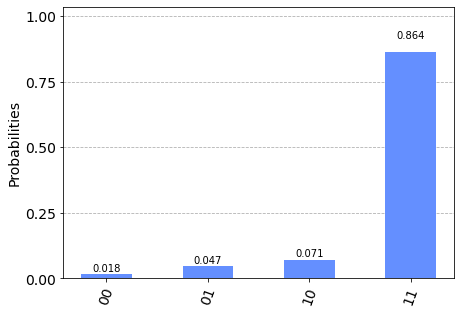
\includegraphics[width=8cm]{grover11.png}
    \caption{Гистограмма, полученная после выполнения кода алгоритма Гровера на квантовом компьютере ibmqx2. Результаты соответствуют теории.}
    \label{fig:grovers_output}
\end{figure}

\subsection{Техническая реализация алгоритма Саймона}\label{appsec:simons}

Задача алгоритма Саймона состоит в том, чтобы при наличии функции $f : \{ 0, 1 \} ^n \to \{ 0, 1 \} ^n$, которая считается инвариантной при наличии некоторой $n$-битной XOR маски $a$, вычислить $a$. Другими словами, при известной $f(x) = f(y)$ и только если $x \oplus y  \in  \{ 0, a \}$, вычислить $a$.

Это может использоваться для построения системы линейных уравнений, которые можно будет использовать для нахождения результатов и вычисления маски XOR определённых функций, которые пимеют многочисленное количество способов применения в криптографии.
\begin{enumerate}
\item Инициализация двух регистров $n$-кубитов в нулевом состоянии.
\begin{equation}
    \lvert \psi_1 \rangle = \ket{0} ^{\otimes n} \ket{0} ^{\otimes n}
\end{equation}

\item Применение преобразования Адамара к первому регистру.
\begin{equation}
    \lvert \psi_2 \rangle = \frac{1}{\sqrt{2^n}} \sum_{x \in \{0,1\}^{n} } \lvert x \rangle\lvert 0 \rangle^{\otimes n}
\end{equation}

\item Применение функции запроса $Q_f$. 
\begin{equation}
    \lvert \psi_3 \rangle = \frac{1}{\sqrt{2^n}} \sum_{x \in \{0,1\}^{n} } \lvert x \rangle \lvert f(x) \rangle
\end{equation}

\item Измерение второго регистра, в результате чего первый регистр приобретает следующую форму:
\begin{equation}
    \lvert \psi_4 \rangle = \frac{1}{\sqrt{2}}  \left( \lvert x \rangle + \lvert y \rangle \right).
\end{equation}

\item Применение преобразования Адамара к первому регистру.
\begin{equation}
    \lvert \psi_5 \rangle = \frac{1}{\sqrt{2^{n+1}}} \sum_{z \in \{0,1\}^{n} } \left[  (-1)^{x \cdot z} + (-1)^{y \cdot z} \right]  \lvert z \rangle
\end{equation}

\item Измерение первого регистра, которое даёт следующий результат:
\begin{equation}
    (-1)^{x \cdot z} = (-1)^{y \cdot z}.
\end{equation}
\end{enumerate}

Результат должен соответствовать строке $z$, которая преобразуется в $ b \cdot z = 0 \text{ (mod 2)} $ и после применения метода исключения Гаусса может использоваться для вычисления маски XOR для функции $f(x)$. 

\begin{verbatim}



"""Код Qiskit для выполнения алгоритма Саймона на квантовом аппаратном обеспечении при наличии 2 кубитов и b = '11'. """

# Импорт Qiskit
from qiskit import IBMQ, BasicAer
from qiskit.providers.ibmq import least_busy
from qiskit import QuantumCircuit, execute

# Импорт базовых инструментов работы с графиками
from qiskit.visualization import plot_histogram
from qiskit_textbook.tools import simon_oracle

# Присвоение b значения '11'
b = '11'

# 1) Инициализация кубитов
n = 2
simon_circuit_2 = QuantumCircuit(n*2, n)

# 2) Применение вентиля Адамара перед передачей запроса оракулу
simon_circuit_2.h(range(n))

# 3) Передача запроса оракулу
simon_circuit_2 += simon_oracle(b)

# 5) Применение вентиля Адамара к входному регистру
simon_circuit_2.h(range(n))

# 3) и 6) Измерение кубитов
simon_circuit_2.measure(range(n), range(n))

# Загрузка сохранённых учётных записей IBMQ и получение доступа к наименее занятому компьютеру базы данных
IBMQ.load_account()
provider = IBMQ.get_provider(hub='ibm-q')
backend = least_busy(provider.backends(filters=lambda x: x.configuration().n_qubits >= n and 
                                   not x.configuration().simulator and x.status().operational==True))
print("least busy backend: ", backend)

# Выполнение и отслеживание работы
from qiskit.tools.monitor import job_monitor
shots = 1024
job = execute(simon_circuit_2, backend=backend, shots=shots, optimization_level=3)
job_monitor(job, interval = 2)

# Получение графиков и построение расчётов
device_counts = job.result().get_counts()
plot_histogram(device_counts)

# Дополнительное применение функции для вычисления скалярного произведения результатов
def bdotz(b, z):
    accum = 0
    for i in range(len(b)):
        accum += int(b[i]) * int(z[i])
    return (accum % 2)

print('b = ' + b)
for z in device_counts:
    print( '{}.{} = {} (mod 2) ({:.1f}%)'.format(b, z, bdotz(b,z), device_counts[z]*100/shots))
    
# Самыми значащими результатами будут те, для которых b dot z=0(mod 2).

'''b = 11
11.00 = 0 (mod 2) (45.0%)
11.01 = 1 (mod 2) (6.2%)
11.10 = 1 (mod 2) (6.4%)
11.11 = 0 (mod 2) (42.4%)'''


Ссылка Github для этого кода:

https://github.com/hamburgerguy/Quantum-Algorithm-Implementations/blob/master/Simon.py

\end{verbatim}

\break 
\begin{figure}
    \centering
    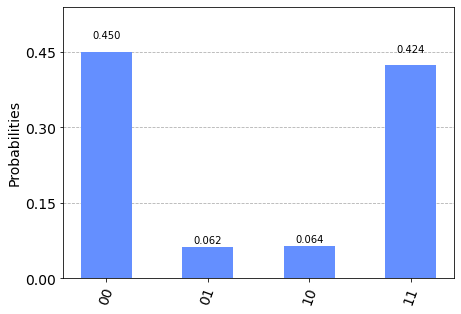
\includegraphics[width=8cm]{simons11.png}
    \caption{Результат выполнения кода алгоритма Саймона на квантовом компьютере ibmqx2. Результаты соответствуют теории.}
    \label{fig:simons_output}
\end{figure}

\bibliography{bibliography}{}
\bibliographystyle{unsrt}



\end{document}